
%!TEX TS-program = xelatex
%!TEX encoding = UTF-8 Unicode
%!BIB TS-program = biber
%!BIB program = biber
\documentclass[12pt,twoside]{book}
%\usepackage{extsizes}
\usepackage{geometry}                 % See geometry.pdf to learn the layout options. There are lots.
\geometry{a4paper}                        % ... or a4paper or a5paper or ...
%\geometry{landscape}                % Activate for for rotated page geometry
%\usepackage[parfill]{parskip}    % Activate to begin paragraphs with an empty line rather than an indent section
\geometry{left=3cm}
\geometry{right=3cm}
\geometry{bottom=2cm}
\geometry{top=2cm}
\usepackage{graphicx}
\usepackage{amssymb}

\usepackage{polyglossia}
\usepackage[babel]{csquotes}
\setdefaultlanguage{german}

\usepackage{titlesec}
\usepackage{hyperref}
\usepackage[all]{hypcap} % Make references jump to the figure and not to the caption.
\usepackage{enumitem}

\usepackage{wasysym}
\usepackage{minted}

\usepackage{booktabs}
\usepackage{tabularx}

\usepackage{todonotes}

\usepackage{float}

\usepackage{tikz}

\usepackage{ifplatform}

\usepackage{savesym}
\savesymbol{iint}
\savesymbol{iiint}
\usepackage{amsmath}

\setlength{\parindent}{0cm}
\setlength{\parskip}{\medskipamount}

% Will Robertson's fontspec.sty can be used to simplify font choices.
% To experiment, open /Applications/Font Book to examine the fonts provided on Mac OS X,
% and change "Hoefler Text" to any of these choices.

\usepackage{fontspec,xltxtra,xunicode}

\ifmacosx
	\newcommand{\romanFont}{Linux Libertine O}
\else
	\newcommand{\romanFont}{Linux Libertine O}
\fi

\defaultfontfeatures{Mapping=tex-text}
\setmainfont[Mapping=tex-text]{\romanFont}
%\setsansfont[Scale=MatchLowercase,Mapping=tex-text]{Gill Sans}
%\setmonofont[Scale=MatchLowercase]{Andale Mono}
% \setmonofont[Mapping=tex-text,%
%     ItalicFont=Source Code Pro ExtraLight,%
%     BoldFont=Source Code Pro]{Source Code Pro Light}

%\newcommand{\HRule}{\rule{\linewidth}{0.1pt}}
%\newcommand{\logoheight}{2.5cm}

\renewcommand{\title}{Enterprise Infoboard - Intelligente Visualisierung und Austausch von heterogenen Informationen im Unternehmen}
\renewcommand{\author}{Tom Nick}
%\date{}                                           % Activate to display a given date or no date

% PDF properties
\hypersetup{
	pdftitle={\title{}},
	pdfauthor={\author{}}
}

\usepackage[
style=numeric,
natbib=true,
backend=biber,
sorting=none
]{biblatex}
\bibliography{bachelorthesis}{}

\setlength{\bibitemsep}{8pt}
%\setlength{\bibhang}{0.2cm}

\usepackage{xpatch}
\xpretobibmacro{author}{\mkbibbold\bgroup}{}{}
\xapptobibmacro{author}{\egroup}{}{}
\xpretobibmacro{bbx:editor}{\mkbibbold\bgroup}{}{}
\xapptobibmacro{bbx:editor}{\egroup}{}{}

\renewcommand*{\labelnamepunct}{\mkbibbold{\addcolon\space}}


\usepackage{changepage}

\makeatletter
\renewcommand{\todo}[2][]{\tikzexternaldisable\@todo[#1]{#2}\tikzexternalenable}
\makeatother

\setcounter{secnumdepth}{3}
\setcounter{tocdepth}{2}

%\newcommand*{\fullref}[1]{\hyperref[{#1}]{\autoref*{#1} \nameref*{#1}}}
\newcommand*{\fullref}[1]{\hyperref[{#1}]{\autoref*{#1} (\nameref*{#1})}}

\newcommand{\makemu}{{\fontspec{Linux Libertine O}μ}}

\usepackage{multirow}

\usepackage{capt-of}

\usepackage[hang,flushmargin,bottom]{footmisc}

\newenvironment{absolutelynopagebreak}
  {\par\nobreak\vfil\penalty0\vfilneg
   \vtop\bgroup}
  {\par\xdef\tpd{\the\prevdepth}\egroup
   \prevdepth=\tpd}

\usepackage{titlesec}

\titleformat{\chapter}[display]
    {\normalfont\huge\bfseries}{\chaptertitlename\ \thechapter}{20pt}{\Huge}
\titlespacing*{\chapter}{0pt}{0pt}{40pt}

\usetikzlibrary{arrows,automata,positioning}

\usepackage{soul}

\usepackage{fancyhdr}
\fancyhead{}
\fancyfoot{}
\fancyhead[RE]{\textsc{\nouppercase{\rightmark}}}
\fancyhead[LO]{\textsc{\nouppercase{\leftmark}}}

\fancyfoot[CO,CE]{\thepage}
\pagestyle{fancy}

\setlength{\headheight}{14.5pt}

\let\cleardoublepage\clearpage

\usepackage[section]{placeins}

\usepackage{afterpage}
\newcommand\blankpage{%
    \null
    \thispagestyle{empty}%
    \addtocounter{page}{-1}%
    \newpage}

\usepackage{listings}


\newcounter{savepage}
\begin{document}

% Titlepage
\begin{titlepage}
%\includegraphics[height=\logoheight,page=1]{Telekom_Logo_bw.pdf} \hfill \includegraphics[height=\logoheight,page=1]{TU_Logo.pdf}
\begin{center}
%\vspace{1cm}
%{\Huge Bachelor}\\
{\Huge \textsc{Technische Universität Berlin}}
{\fontsize{2.5cm}{2cm}\selectfont \textsc{Bachelor Thesis}\par}
\vspace{1cm}
\hrule
\vspace{0.3cm}
{\Huge \textsc{\title{}}\par}
~\\[0.1cm]
{\Large Supervisor: Prof. Dr. Dr. h.c. Albayrak}\\[0.1cm]
{\Large Advisors: Dipl.-Inform. Michael Meder}\\[0.3cm]
{\Large Geschrieben von \author{}}\\[0.1cm]
{\Large \today}
\vspace{0.55cm}
\hrule
\end{center}
%\vspace{1cm}
\vfill
\begin{center}{\Large\textbf{Abstrakt}}\end{center}

Das DAI-Labor (Distributed Artificial Intelligence) ist eine der führenden Forschungseinrichtungen im Bereich verteilte Suchmaschinen - welche nun nicht mehr reine Forschung sind, sondern wie deren PIA-System (Personal Information Assistant) von zahlreichen Verwaltungen als Alternative zu privaten Suchmaschinen benutzt wird. Eine interessante Aufgabe besteht darin, die Suchergebnisse von verschiedenen Suchmaschinen zusammenzuführen und für den Suchenden in einem visuell einheitlichen Format darzustellen. In dieser Arbeit wird eine Visualisierung in der Art einer \textit{Social Media Wall} untersucht und realisiert.
Ein weiteres Themengebiet des DAI-Labors ist die Gamification im Enterprise Bereich. Auch diese Mechanismen werden untersucht und benutzt, um die Benutzung der Applikation zu fördern.
Ausführlich wird auf die neuen Entwicklungsmethoden im Bereich der Webapplikationen eingegangen und aufgezeigt, wie diese die Entwicklung der Applikation vereinfachen und verbessern können.
Das Ergebnis dieser Arbeit ist eine funktionsfähige und mit neuesten Methoden entwickelte Webapplikation, die ein neuartiges Interface für Suchergebnisse unterschiedlicher Herkunft besitzt und deren Benutzung durch nahtlos eingebundene Spielelemente gefördert wird.

\end{titlepage}

\pagenumbering{roman}

%\blankpage

\chapter*{Declaration of authorship}\addcontentsline{toc}{chapter}{Eidesstatliche Erklärung}

I hereby certify that the thesis I am submitting is entirely my own original work except where otherwise indicated. I am aware of the University's regulations concerning plagiarism, including those regulations concerning disciplinary actions that may result from plagiarism. Any use of the works of any other author, in any form, is properly acknowledged at their point of use.\footnote{The template for this declaration of authorship was taken from \url{https://www.wiwi.hu-berlin.de/international/mems/upload/authorship}.}

\vspace{2cm}

Berlin, \today\\
\textbf{Place, date}\hfill\textbf{Signature}
\cleardoublepage

\tableofcontents
\newpage

\setcounter{savepage}{\arabic{page}}
\pagenumbering{arabic}

\chapter{Einleitung}

Die gemeinsame Darstellung von Inhalten aus verschiedenen Quellen ist ein interessantes und weit erforschtes Thema. Die Idee ist, dem Benutzer die Benutzung bzw. die Konsumierung von Inhalten angenehmer und effizienter zu gestalten, indem ein einheitliches Interface für Inhalte geschaffen wird. Vor der \textit{digitalen Revolution} war das ein äußerst aufwendiges und kostspieliges Unterfangen \footnote{Vergleich hier zu der Encyclopædia Britannica
und Wikipedia, letztere konnte in wenigen Jahren mehr Inhalte mit gleicher Qualität aggregieren, also das Traditionsunternehmen in 200 Jahren \cite{giles2005internet}.}. Als Beispiel seien die frühen Enzyklopädien genannt, welche versuchten, sämtliches Wissen an einem Ort in homogener Sprache und Darstellung bereitzustellen. Durch die momentan verfügbaren Technologien ist das Erstellen einer einheitlichen Datenquelle für verschiedene Inhalte deutlich einfacher geworden. Die Schwierigkeit einer qualifizierten Zusammenführung besteht dennoch weiter. Produkte die diese Aufgabe entsprechend lösen sind sehr erfolgreich. Wie zum Beispiel Facebook mit der Aggregation von sozialen Aktivitäten.

Wenn man sich jedoch auf eine Teilmenge der verfügbaren Informationen beschränkt, wie Nachrichten die als RSS (Rich Site Summary) verfügbar sind, ist es deutlich einfacher eine angemessene Zusammenstellung der Inhalte zu gestalten. Prominentes Beispiel für eine Anwendung dieser Art ist die Nachrichten-Applikation pulse \cite{pulse}, die auf Basis von RSS ein angenehmes und attraktives Interface für die gleichzeitige Konsumierung mehrerer Nachrichtenseiten anbietet. Der Erfolg von \textit{pulse} spricht mit ca. 22 Millionen Downloads auf dem Android-System für sich.

Eine der komplexesten Zusammenführungen von Informationen unterschiedlichster Art stellen Suchmaschinen da, da hier eine Reduzierung der benutzten Informationen, eine sofortige Verschlechterung der Suchergebnisse bewirkt - die ideale Suchmaschine würde jede mögliche Datenquelle und jedes existierende Dateiformat indizieren.
Suchmaschinen der Gegenwart versuchen sich diesem Optimum immer weiter zu nähern und können mittlerweile eine Vielzahl an Datenformaten und Datenquellen nutzen und verarbeiten.
Trotz der beinahe unendlichen Diversität der indizierten Daten werden die Suchergebnisse meistens über eine einfache Auflistung in Textform dargestellt, weil jedes Dateiformat mehr oder minder auf Text reduziert werden kann.

Neue Visualisierungsformen für Suchergebnisse sind bisher überraschenderweise wenig untersucht worden. Andere Bereiche sind auf diesem Gebiet experimentierfreudiger, wie zum Beispiel die \textit{Social Media Walls} mit der Zusammenführung von Social-Media-Kanälen.
Sie sind eine Form der Darstellung für Inhalte mit kurzen Texten und Bildern aus verschiedenen sozialen Kanälen. Die Besonderheit liegt in der Homogenisierung der Inhalte und in der gleichzeitigen Darstellung von verschiedenen Kanälen.
Suchergebnisse besitzen ganz ähnliche Attribute wie die Datenpunkte von Social-Media-Kanälen, womit die Frage nahe liegt, ob die Visualisierung von Suchergebnissen verbessert werden kann, indem eine ähnliche Darstellung wie der von \textit{Social Media Walls} benutzt wird.
Diese Arbeit bemüht sich diese Frage zu beantworten und eine neue Visualisierungsform für Suchergebnisse zu finden mit der Inspiration von \textit{Social Medial Walls}.

Der Einsatz von Gamification hat in den letzten Jahren stetig zugenommen, da es ein effektives Mittel ist, um das Erlebnis des Nutzers zu erhöhen und seine Interaktionen mit der Applikation zu fördern.
Die Benutzung von Gamification im Enterprise-Bereich bzw. in kleinen sozialen Kreisen ist bisher noch nicht allzu populär. Die prominentesten Beispiele sind Sport-Apps, wie Strava \cite{strava} oder Nike+ \cite{nike}, bei denen Freunde sich miteinander vergleichen können. Eine Integration von Gamification stellt damit in diesem Bereich eine interessante Herausforderung dar, da deren Potential bisher noch nicht vollständig geklärt ist.

\section{Beschreibung des Infoboards}

Das Infoboard ermöglicht die Abrufung von Informationen aus heterogenen Unternehmensquellen. Hierzu kann der Benutzer nach Informationen mittels verschiedener Themen suchen. Es können jederzeit Themen entfernt oder hinzugefügt werden. Die gleichzeitige Anzeige mehrerer Themen hat die Motivation, dass der Benutzer bei der Suche von Themenübergreifenden Informationen diese schneller und komfortabler finden kann.
Die Informationen können binär bewertet werden, womit sie global in der Relevanz steigen.
Durch die gezielte Benutzung von Gamification-Elementen wird versucht die Anzahl an Bewertungen durch den Benutzer zu erhöhen.
Durch die Bewertungen soll die Qualität der Relevanz der Information verbessert werden, womit eine Verbesserung des unternehmensinternen Informationsaustausches angestrebt wird.


\section{Anforderungen}

Im Folgenden werden die Anforderungen zur Entwicklung des Infoboards aufgelistet. Diese waren jedoch anfangs größtenteils noch offen. Die genauen Spezifikationen haben sich erst während der Ausarbeitung ergeben.

\begin{description}

\item[Darstellung von Daten]

Eine der Hauptanforderungen ist die Darstellung von heterogenen Informationen (im zukünftigen Verlauf des Textes wird sie als Kacheln bezeichnet) im Stil einer \textit{Social Media Wall}. Daraus folgen weitere Ansprüche, zum Beispiel dass es unterschiedliche Kacheln gibt - also für verschiedene Informationen verschiedene Darstellungen. Kacheln für Informationen wie Kontakte und Webseiten können ganz unterschiedlich aufgebaut sein. Die dargestellten Inhalte sind weiterhin dynamisch, während des Betriebes können Kacheln hinzukommen, entfernt oder anderen Themen zugeordnet werden. Die Kacheln bieten zudem Interaktionsmöglichkeiten, da sie bewertet und favorisiert werden können.

\item[Bewertungssystem]

  Der Benutzer soll in der Lage sein, angezeigte Suchergebnisse zu bewerten und dadurch die Priorisierung von Suchergebnissen zukünftiger Anfragen für \textbf{alle} Benutzer zu verändern.

\item[Benutzung mehrerer heterogener Datenquellen]
  Die angezeigten Informationen können aus mehreren Datenquellen kommen, das heißt die gleichzeitige Darstellung von Informationen von zum Beispiel Facebook mit denen von Twitter. Auch hier ist wichtig, dass zusätzliche Datenquellen hinzufügt werden können.

\item[Authentifizierungssystem]
	Zur Benutzung der Gamification-Elemente und der Suchanfrage bedarf es einer Authentifizierung. Die Suchergebnisse können unternehmensinterne Dokumente enthalten, deswegen muss sichergestellt werden, dass kein Benutzer der nicht authentifiziert ist, Zugriff auf die Applikation hat.

\item[Single Page Application]
  Es soll eine sogenannte \textit{Single Page Application} erstellt werden, das heißt eine Webapplikation bei der JavaScript abseits des initialen Seitenaufrufes alles rendert. Im Gegensatz zur klassischen Methodik, bei der jede Interaktion in einer komplett neuen Seite, die vom Server gerendert wird, resultiert \cite{mesbah2007migrating}.

\item[Gamification]
  Um zur Benutzung der Seite zu animieren sollen Gamification-Methoden eingeführt werden wie zum Beispiel Punkte für das tägliche einloggen bis hin zu erweiterten Methoden wie der Erstellung eines Compulsion Loop. ``Der Compulsion Loop ist eine modellierte Kette an Aktivitäten, die gewohnheitsmäßig wiederholt werden, um eine neurochemische Belohnung zu erhalten'' (\cite{gamasutra}, übersetzt aus dem Englischen).

\item[Konfiguration]
  Es muss möglich sein eine Vielzahl an Parameter anzupassen, einige davon dienen auch als Benutzerinterface für den Benutzer andere wiederum als simple Konfigurationsdatei für verwendete URLs und ähnliches.

\end{description}

\section{Relevante Arbeiten}

Da es Bestandteil dieser Arbeit ist, Erkenntnisse aus verschiedenen Gebieten zu Aggregieren, gibt es keine direkt zu Grunde liegenden Arbeiten. Vielmehr werden Erkenntnisse verschiedener Bereiche untersucht und zusammengeführt.

\subsection{Social Media Walls}

% TODO
Im folgenden werden verschiedene Angebote von \textit{Social Media Walls} untersucht um Unterschiede und Gemeinsamkeiten dieser festzustellen.

Eine sehr gute Auflistung verschiedener \textit{Social Media Wall}-Applikationen bietet \citep{hofram}. Die Homogenität dieser Angebote ist jedoch erstaunlich. Würde man die Produkte zweier verschiedener Anbieter nebeneinander sehen, wären die größten Unterschiede stilistischer Natur wie etwa die benutzten Farbschemas und Schriftarten. Leider sind die wenigsten Produkte in einer Demo zu testen, da die Lösungen üblicherweise auf den Kunden zugeschnitten werden. Primärer Use-Case sind große Veranstaltungen wie Konzerte, weswegen auch keine im Produktiveinsatz eingesehen werden konnten. In Abbildung \ref{fig:socialwall} kann eine der Implementierungen gesehen werden.\\

\begin{figure}[htbp]
    \centering
    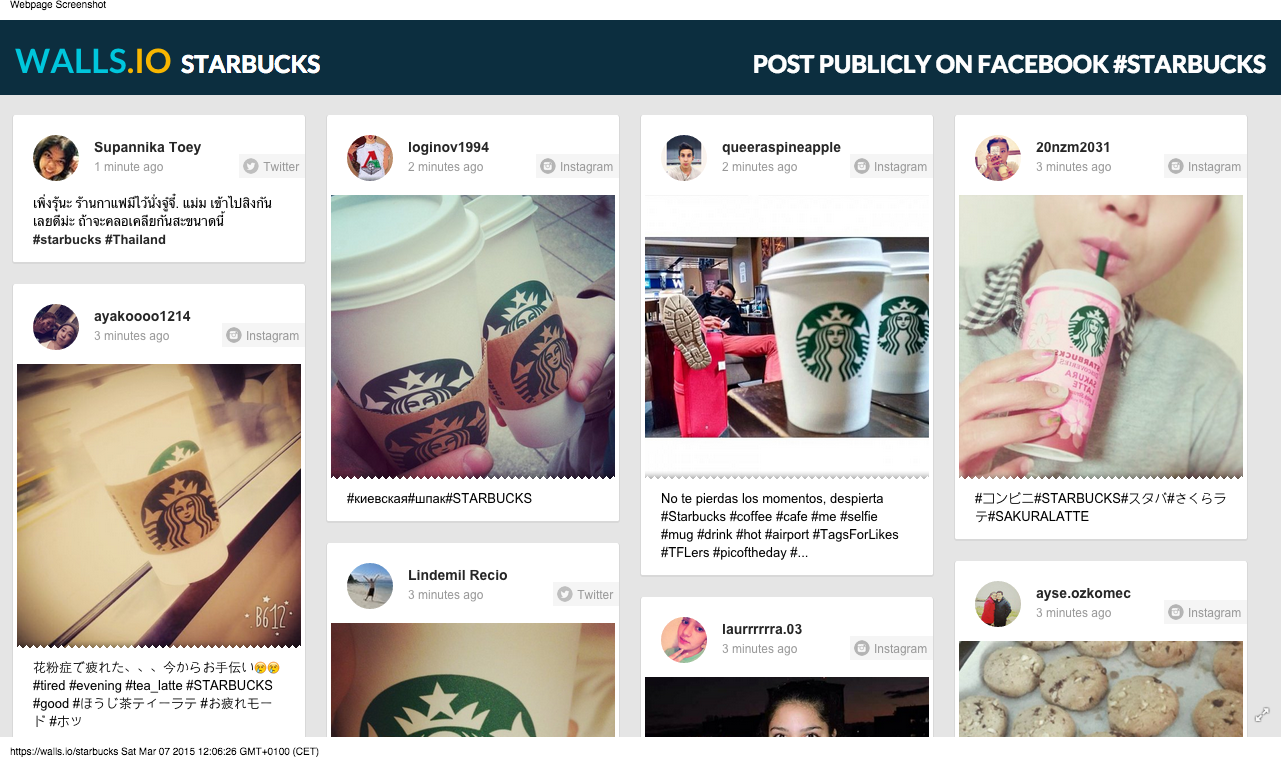
\includegraphics[width=0.8\textwidth]{images/Starbucks.png}
    \caption{Eine \textit{Social Media Wall} vom Anbieter walls.io \cite{wallsio}}\label{fig:socialwall}
\end{figure}

Da die dargebotenen Angebote sehr ähnlich sind, wird in dieser Arbeit nicht weiter auf alle Anbieter eingegangen. Die Darstellungsform ist aber dennoch weiterhin interessant und wird als grobe Inspiration die Darstellung der Suchergebnisse dienen.


\subsection {Gamification}\label{sec:intro_game}

Neben der Visualisierung  von Informationen aus heterogenen Unternehmensquellen, ist Gamification der zweite große Aspekt der Applikation. Wie in der Einleitung erwähnt, ist Gamification eine mittlerweile weitverbreitete und äußerst effektive Technik, um das sogenannte \textit{User-Engagement} zu erhöhen. Allein durch Gamification konnte die Seite DevHub ihre \textit{Engagement}-Rate um 20\% steigern \citep[pp. 17]{zichermann2011gamification}. Zahlreiche StartUps feiern große Erfolge mit dem Hinzufügen von Gamification zu anstrengenden oder langweiligen Aufgaben, wie das Lernen einer Sprache (Duolingo\footnote{https://de.duolingo.com/}) oder Programmieren (Codecademy\footnote{http://www.codecademy.com/}).

Der Begriff Gamification entstand erst 2008 und hat seitdem viele Bedeutungen erlangt. Deterding \cite{deterding2011game} bemühte sich eine einheitliche Definition zu finden, die auch im folgenden Kontext verwendet wird: ``Gamification is the use of game design elements in non-game contexts'' \citep{deterding2011game}.

Das Infoboard dient als Interface für den Benutzer die heterogenen Unternehmensquellen komfortabel zu benutzen, welches zu besserem Wissensaustausch führen soll. Dies ist offensichtlich ein nicht-Spiele-Kontext der durch erhöhte Benutzerbeteiligung positive Effekte für ein Unternehmen erzielen kann.
Mit dem Einsatz von Gamification-Elementen werden von uns zwei Ziele verfolgt: einerseits soll durch die Verspielisierung der Applikationsmechaniken deren Benutzung erhöht bzw. ein konstanteres \textit{User-Engangement} erzielt werden, andererseits sollen die Mechaniken zur Bewertung der Suchergebnisse gefördert werden, wodurch diese noch besser werden.

Im Folgenden werden bisherige Arbeiten analysiert, die ähnliche Inhalte anzeigen, und Gamification implementiert haben.

Einen schwachen aber effektiven Ansatz verfolgt die Social-News-Seite reddit \cite{reddit}. Jegliche Inhalte (eingereichte Links, Kommentare) der Seite können binär bewertet werden (im reddit-jargon wird hier von \textit{upvotes} und \textit{downvotes} gesprochen). Reicht man nun selbst etwas ein und andere Benutzer bewerten den eingereichten Inhalt, wird die Differenz aus \textit{upvotes} und \textit{downvotes} einem als Karma gutgeschrieben. Wie in klassischen Spielen hat Karma einen endogenen Wert \citep[pp. 21 - 22]{costikyan2005have}, das heißt der Wert besitzt keinerlei Wert außerhalb des Systems, in diesem Falle außerhalb von reddit.

Eine Analyse reddits im Spielekontext führte \cite{massanari2013playful} durch und zeigte auf, dass viele Muster reddits Teil eines Spiels aufbauend auf Karma sind, die die Nutzung und Nutzer reddits weitreichend formten.
Dies zeigt, dass Gamification ein großer Teil reddits, und damit auch dessen Erfolgs ist. Laut der Webanalyseplattform Alexa ist reddit die 32 meist besuchte Webseite der Welt, in den USA ist sie sogar auf Platz 10 \cite{alexa}.
Doch besitzt die Gamification reddits auch negative Seiten, so legt \citep{richerichkarma}  dar, das eine Anhäufung Karmas zum Zweck der Selbstbestätigung der eigenen Meinung betrieben wird. Benutzer reddits werden darauf gepolt ihre eingereichten Beiträge anhand der Höhe des Karmas, welches der Beitrag voraussichtlich liefern wird, auszusuchen - und nicht anhand Qualität oder Relevanz.

DAIKnow \citep{meder2014daiknow} ist eine Bookmarking Seite wie auch delicous.com \cite{delicious}, bei der Links mit Beschreibungen und Keywords eingereicht werden können. Durch den gezielten Einsatz von Punkten, Abzeichen und Bestenlisten wird die Benutzung der Seite gesteigert. Im Gegensatz zu reddit ist dieses System jedoch weitaus komplexer, so bekommt der Benutzer unter anderem Punkte für den täglichen Aufruf, Punkte für das Einrechen eines Links oder das ein andere Benutzer seinen Link kopiert hat.
Ein Problem des Konzeptes von DAIKnow ist, dass häufige Benutzer alle verfügbaren Abzeichen freischalteten und damit der Gamification-Aspekt abgeschwächt wurde, da keine neuen Abzeichen hinzugefügt wurden.

Die Untersuchung zeigt, dass Gamification bei den Beispielen erfolgreich eingesetzt wird, und bei reddit ein so integraler Bestandteil der Seite ist, dass viele Nutzungsmuster auf reddit davon komplett abhängig sind. Daraus leiten wir ab, dass Gamification einen positiven Nutzen für das Infoboard erzielen kann. Allerdings ist damit nicht endgültig geklärt wie die Gamification im Detail implementiert wird, da das Infoboard im Gegensatz zu reddit oder DAIKnow, keine Möglichkeit besitzt eigenen Inhalt einzureichen. Die genaue Spezifikation der Gamification wird in \ref{chap:game} erarbeitet.

\chapter{Konzeptuelle Umsetzung}\label{chap:concept}

Einer der wichtigsten Aspekte von Interface-getriebenen Applikationen ist das Nutzererlebnis \citep[8 - 17]{garrett2010elements}. In diesem Kapitel werden die zwei Hauptmerkmale dieser Arbeit, die für das Nutzererlebnis wichtig sind analysiert: Gamification und die Visualisierung der Informationen. Auf dieser Basis wird ein Konzept vorgestellt, welches in Kapitel \ref{chap:tech} umgesetzt wird.

\section{Visualisierung der Informationen}\label{chap:concept:wall}

 Wie \cite{bostock2011d3} gezeigt hat, erlauben heutige Webtechnologien nahezu uneingeschränkte Möglichkeiten Daten zu visualisieren. Abseits von der initialen Idee, eine Darstellung ähnlich einer \textit{Social Media Wall} zu benutzen, gibt es eine Vielzahl von Parametern, die betrachtet werden müssen: Das Layout, die Animationen und das Design der individuellen Information.

\subsection{Layout}

Wie Pinterest \cite{pinterest} oder das Metro-Design von Microsoft zeigen, ist ein auf Kacheln  basierendes Layout aktuell eine der populärsten Darstellungen für Medieninhalte verschiedener Art, siehe Abbildung \ref{fig:metro_pinterest}.

\begin{figure}[htbp]
    \centering
    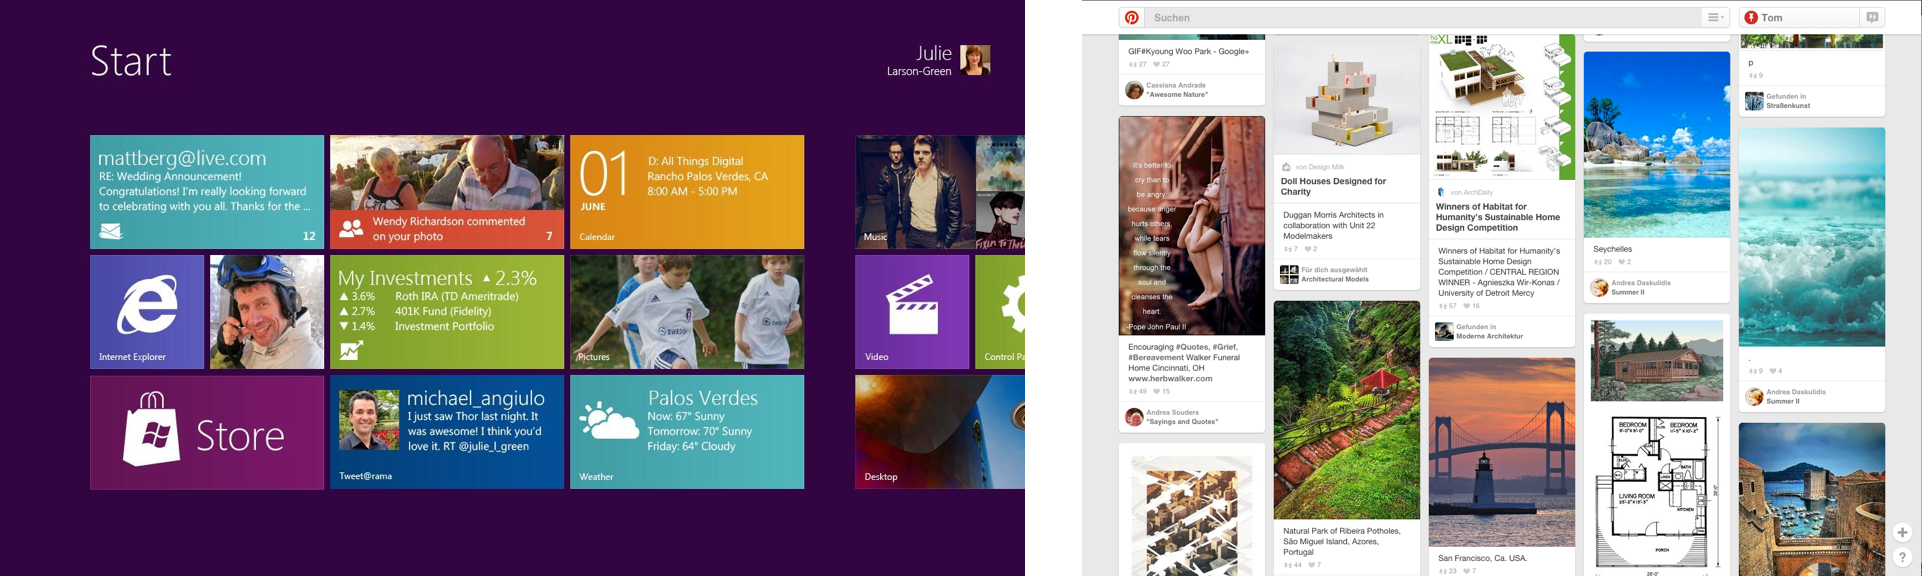
\includegraphics[width=1.0\textwidth]{images/metro_pinterest.png}
    \caption{Links das Rasterbasierte Layout von Windows 8 \cite{metrodesign}, rechts das spaltenbasierte Layout von Pinterest.}
    \label{fig:metro_pinterest}
  \end{figure}

Oft existiert eine Regel, nach welchem Muster die Kacheln angeordnet werden. Zum Beispiel sind die neuesten Kacheln an oberster Stelle positioniert,  oder \textit{wichtigere} Kacheln werden prominenter dargestellt.  Die Kacheln für das Infoboard unterliegen der Regel, dass sie anhand ihrer Wertung (Relevanz + Nutzerbewertung) angeordnet werden müssen. Die folgende Analyse wird deshalb auf das Verhaltensmuster des Layouts fokussiert sein, für den Fall dass Kacheln hinzukommen/wegfallen und damit neu sortiert werden müssen. Dies ist ein normaler Anwendungsfall des Infoboards und tritt immer dann auf wenn der Benutzer Informationen zu einem Thema abfragt oder diese Abfrage wieder löscht.
Im folgenden wird die rasterbasierte mit der spaltenbasierten Darstellung der Kacheln verglichen.

\begin{itemize}
  \item \textbf{Spaltenbasierte Anordnung} \\
  Bei dieser Form werden die einzelnen Kacheln mit einheitlicher Breite und variabler Höhe in Spalten in der Größenordnung von 3-5 dargestellt, siehe Abbildung {fig:column}.

  \begin{figure}[htbp]
    \centering
    \includegraphics[width=0.5\textwidth]{images/livewall_columns.pdf}
    \caption{Spaltenbasierte Anordnung der Inhalte}
    \label{fig:column}
  \end{figure}

  \textbf{Vorteile} \\
  Die Vorteile liegen in der Simplizität der Implementierung und der Intuitivität des Inhaltflusses. Neuer Inhalt wird oben eingefügt und älterer Inhalt rutscht nach unten, wobei je neu hinzugekommener Kachel jeweils nur eine Spalte verrutscht.
  Weiterhin ermöglicht die variable Höhe viel Flexibilität beim Anzeigen des Inhalts - zum Beispiel können lange Texte angemessen angezeigt werden, ohne die Zeichenanzahl zu begrenzen oder ähnliche Limitierungen einzuführen.

  \textbf{Nachteile}\\
  Der größte Nachteil ist die Starrheit des Layouts. Da alle Objekte die gleiche Breite haben ist man stark limitiert wie man die Inhalte darstellt. Abstriche müssen auch gemacht werden bei der Sortierung der Inhalte. Sobald die angezeigten Kacheln einer Sortierung unterliegen, kann der Inhaltsfluss nicht optimal funktionieren. Siehe Abbildung \ref{fig:livewall_sort} für eine detaillierte visuelle Erklärung.

  \begin{figure}[htbp]
    \centering
    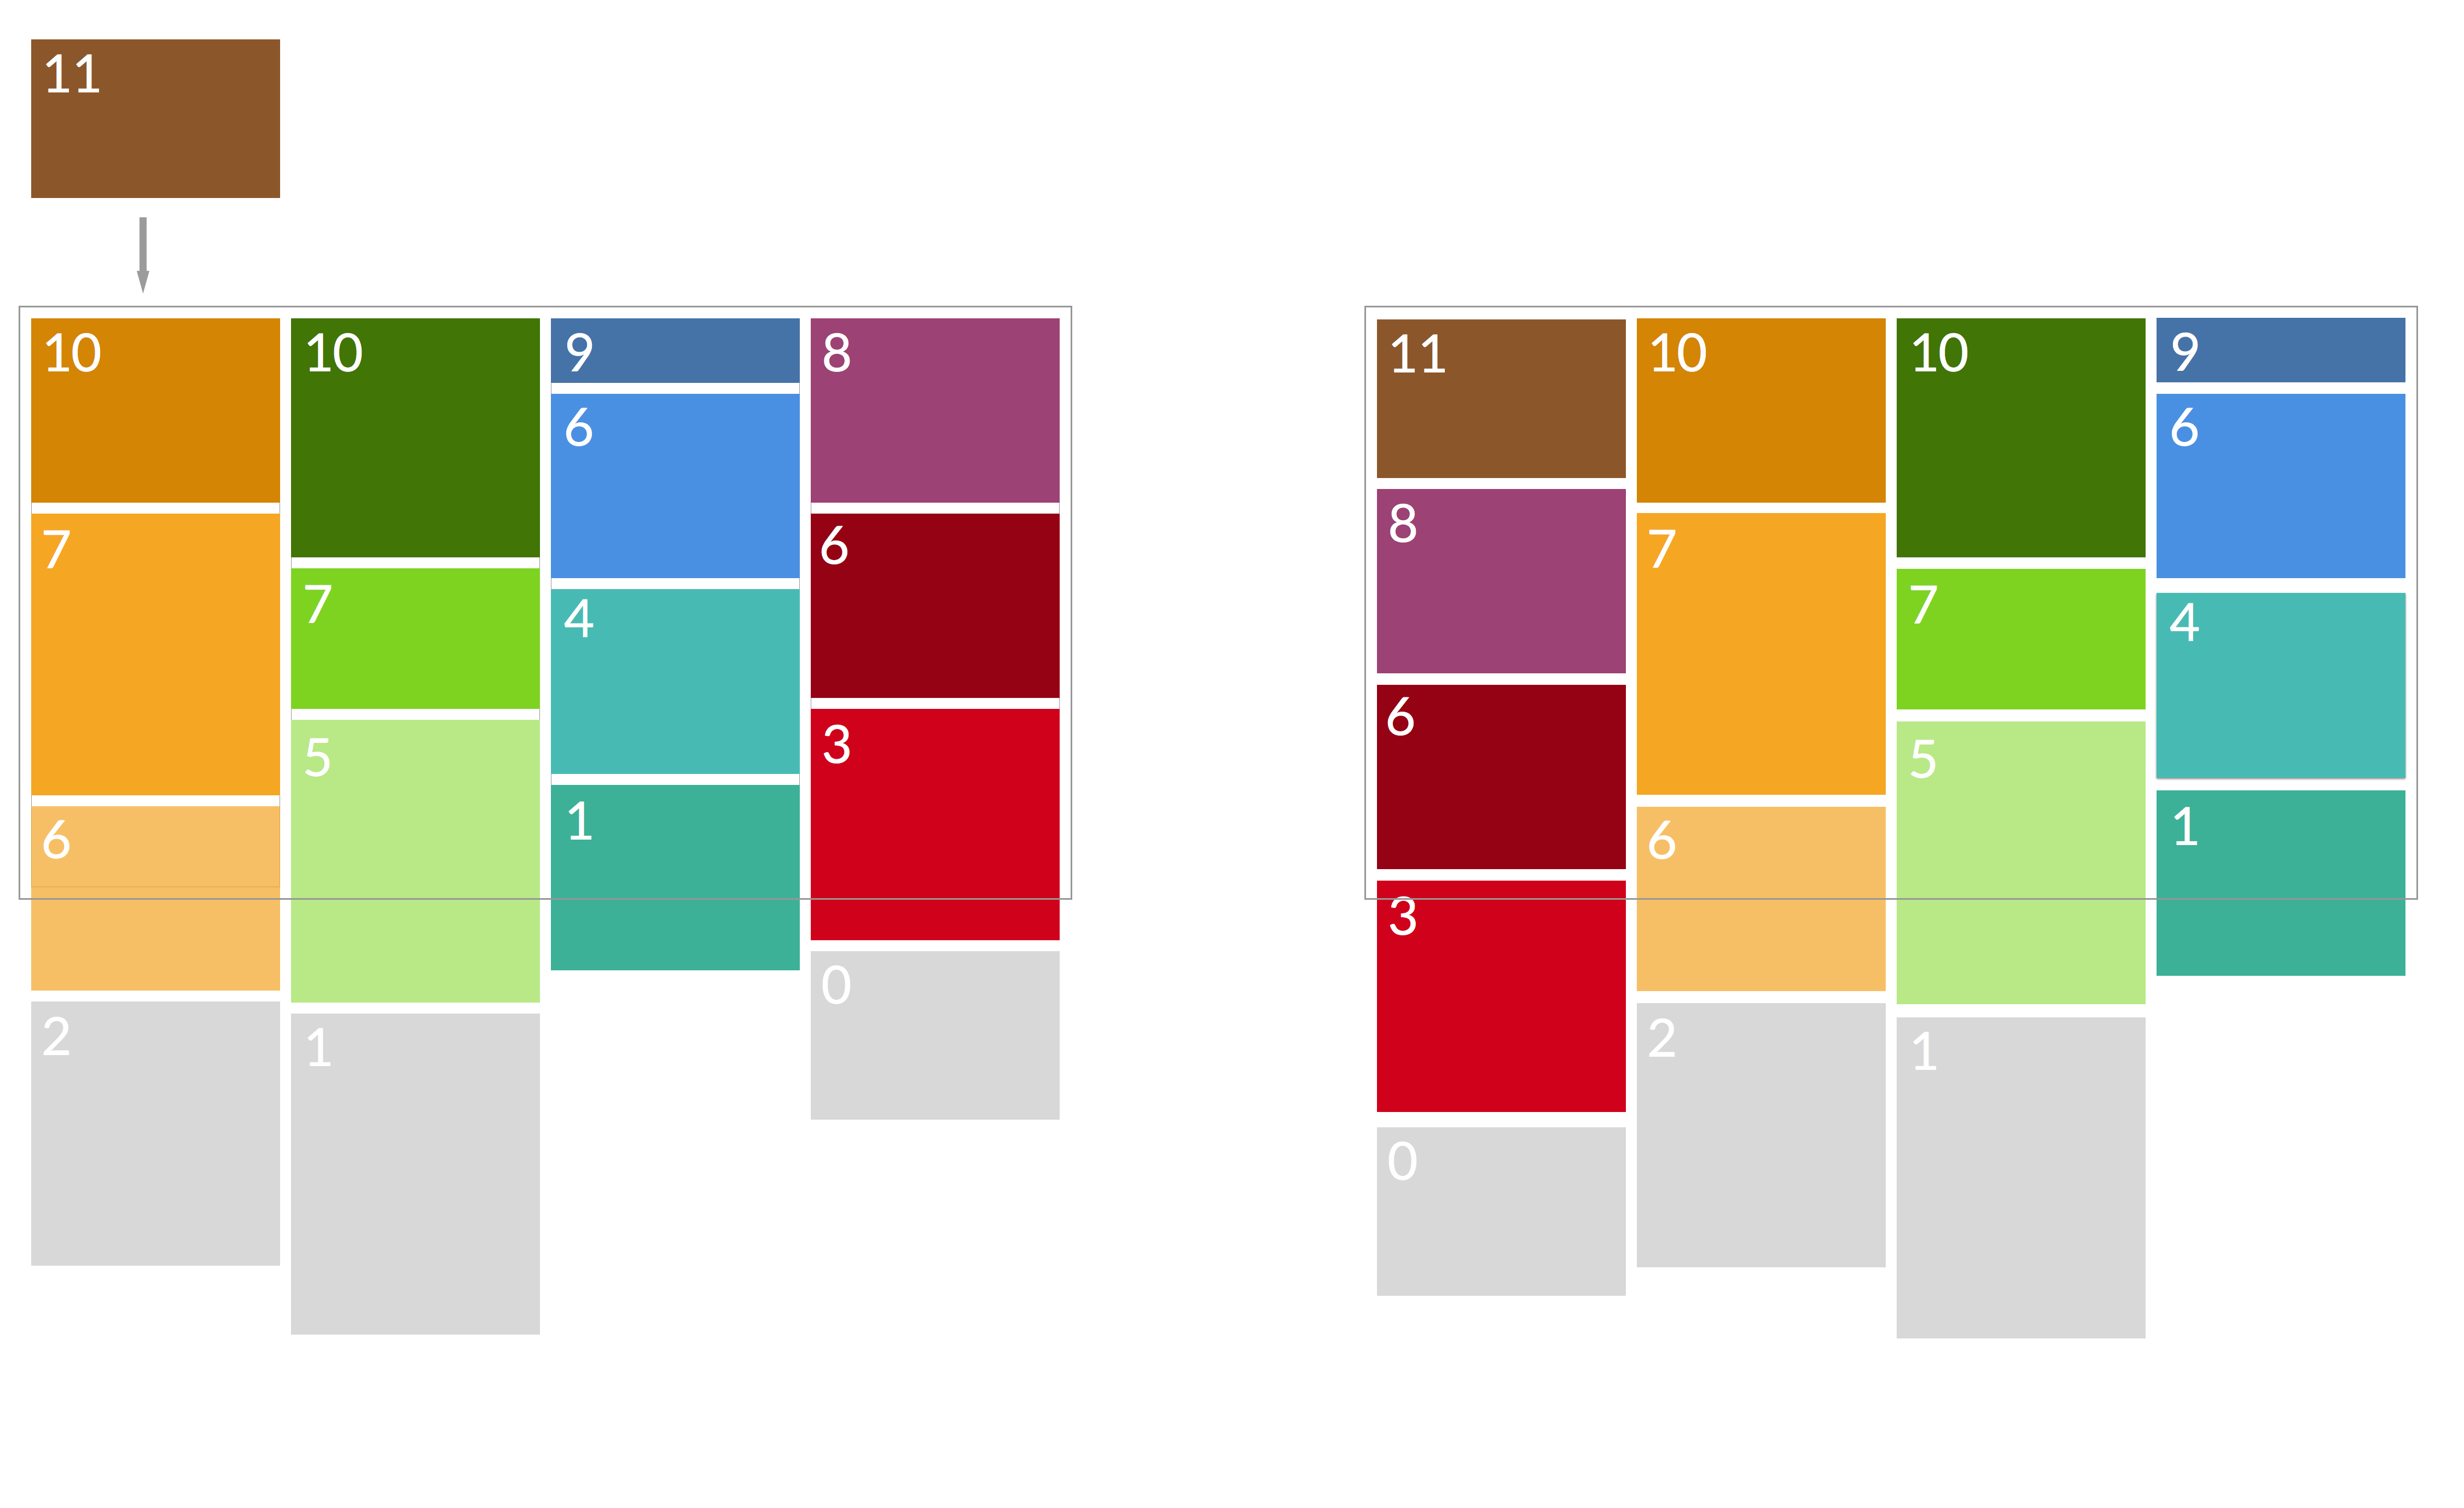
\includegraphics[width=1.0\textwidth]{images/livewall_sort.png}
    \caption{Links wird eine neue Kachel eingefügt die den höchsten Wert besitzt von allen Kacheln, rechts ist das Ergebnis bei Beibehaltung der Sortierung von links nach rechts.}
    \label{fig:livewall_sort}
  \end{figure}

Man kann den optimalen Fluss nur beibehalten indem man die Sortierung Spaltenweise gliedert, dazu müssen jedoch die Kacheln auf eine Spalte festgesetzt werden zum Beispiel mittels einer Hash-Funktion. Dadurch kann aber eine korrekte Sortierung nicht beibehalten werden, wodurch die Güte dieser vom Zufall abhängig und den Benutzer irritieren kann.

  \item \textbf{Rasterbasierte Anordnung}
  Bei dieser Form werden die einzelnen Datenpunkte in einem einheitlichen Raster dargestellt, das heißt die darstellende Fläche wird in einem Raster der Größe $(a, b)$ unterteilt, die Kacheln können nun die Größe $(x, y)$ mit $ x \in \{1, \dots, a, y \in 1, \dots, b\}$ besitzen, siehe Abbildung \ref{fig:raster}.

  \begin{figure}[htbp]
    \centering
    \includegraphics[width=0.8\textwidth]{images/livewall_grid.pdf}
    \caption{links: Das Raster des Grids, rechts: eine zufällige Benutzung des Grids}
    \label{fig:raster}
  \end{figure}

  \textbf{Vorteile} \\
  \begin{itemize}
    \item Ansprechendes Aussehen
    \item Bedeutung kann durch die Größe der Kachel dargestellt werden
    \item Unterschiede in der Darstellung gleicher Datenpunkte durch unterschiedliche Größe
    \item Vorteilhaft bei der Anzeige ohne Interaktion, da es keine abgeschnittenen Inhalte gibt wie beim Spaltendesign
  \end{itemize}

  \textbf{Nachteile}\\
  \begin{itemize}
    \item komplexes Fluss-Verhalten bei neuem Inhalt.
    \item Es müssen komplexere Methoden benutzt werden um Löcher zu verhindern
    \item Es müssen Darstellungen für die verschiedenen Kachelgrößen erstellt werden
    \item unterschiedliche Darstellungsformen können unübersichtlich wirken
  \end{itemize}

\end{itemize}

  \subsection{Probleme beim Flussverhalten}
  Das Flussverhalten beim Einfügen neuer Inhalte ist bei einem Grid-basierten Layout mit unterschiedlichen Kachelgrößen äußerst komplex. Zunächst müsste das Behälterproblem gelöst werden\footnote{Dies ist nötig damit die minimale Anzahl an Lücken entstehen.}, und im zweiten Schritt müssten die Kacheln anhand ihrer Bewertung nochmals sortiert werden. Die Lösungen des Behälterproblems so zu optimieren, dass der optische Fluss der Kacheln minimiert wird, ist von derartiger Komplexität, dass dies nicht in Betracht gezogen werden kann. Die JavaScript-Bibliothek packery \cite{packery} implementiert den ersten Schritt und ordnet die Kacheln anhand einer Lösung des Behälterproblems. Anhand der packery-Methode \texttt{prepend} kann sehr gut erahnt werden, dass der Fluss nicht einfach nachvollziehbar ist, siehe Abbildung \ref{fig:grid_flow}.

  \begin{figure}[htbp]
    \centering
    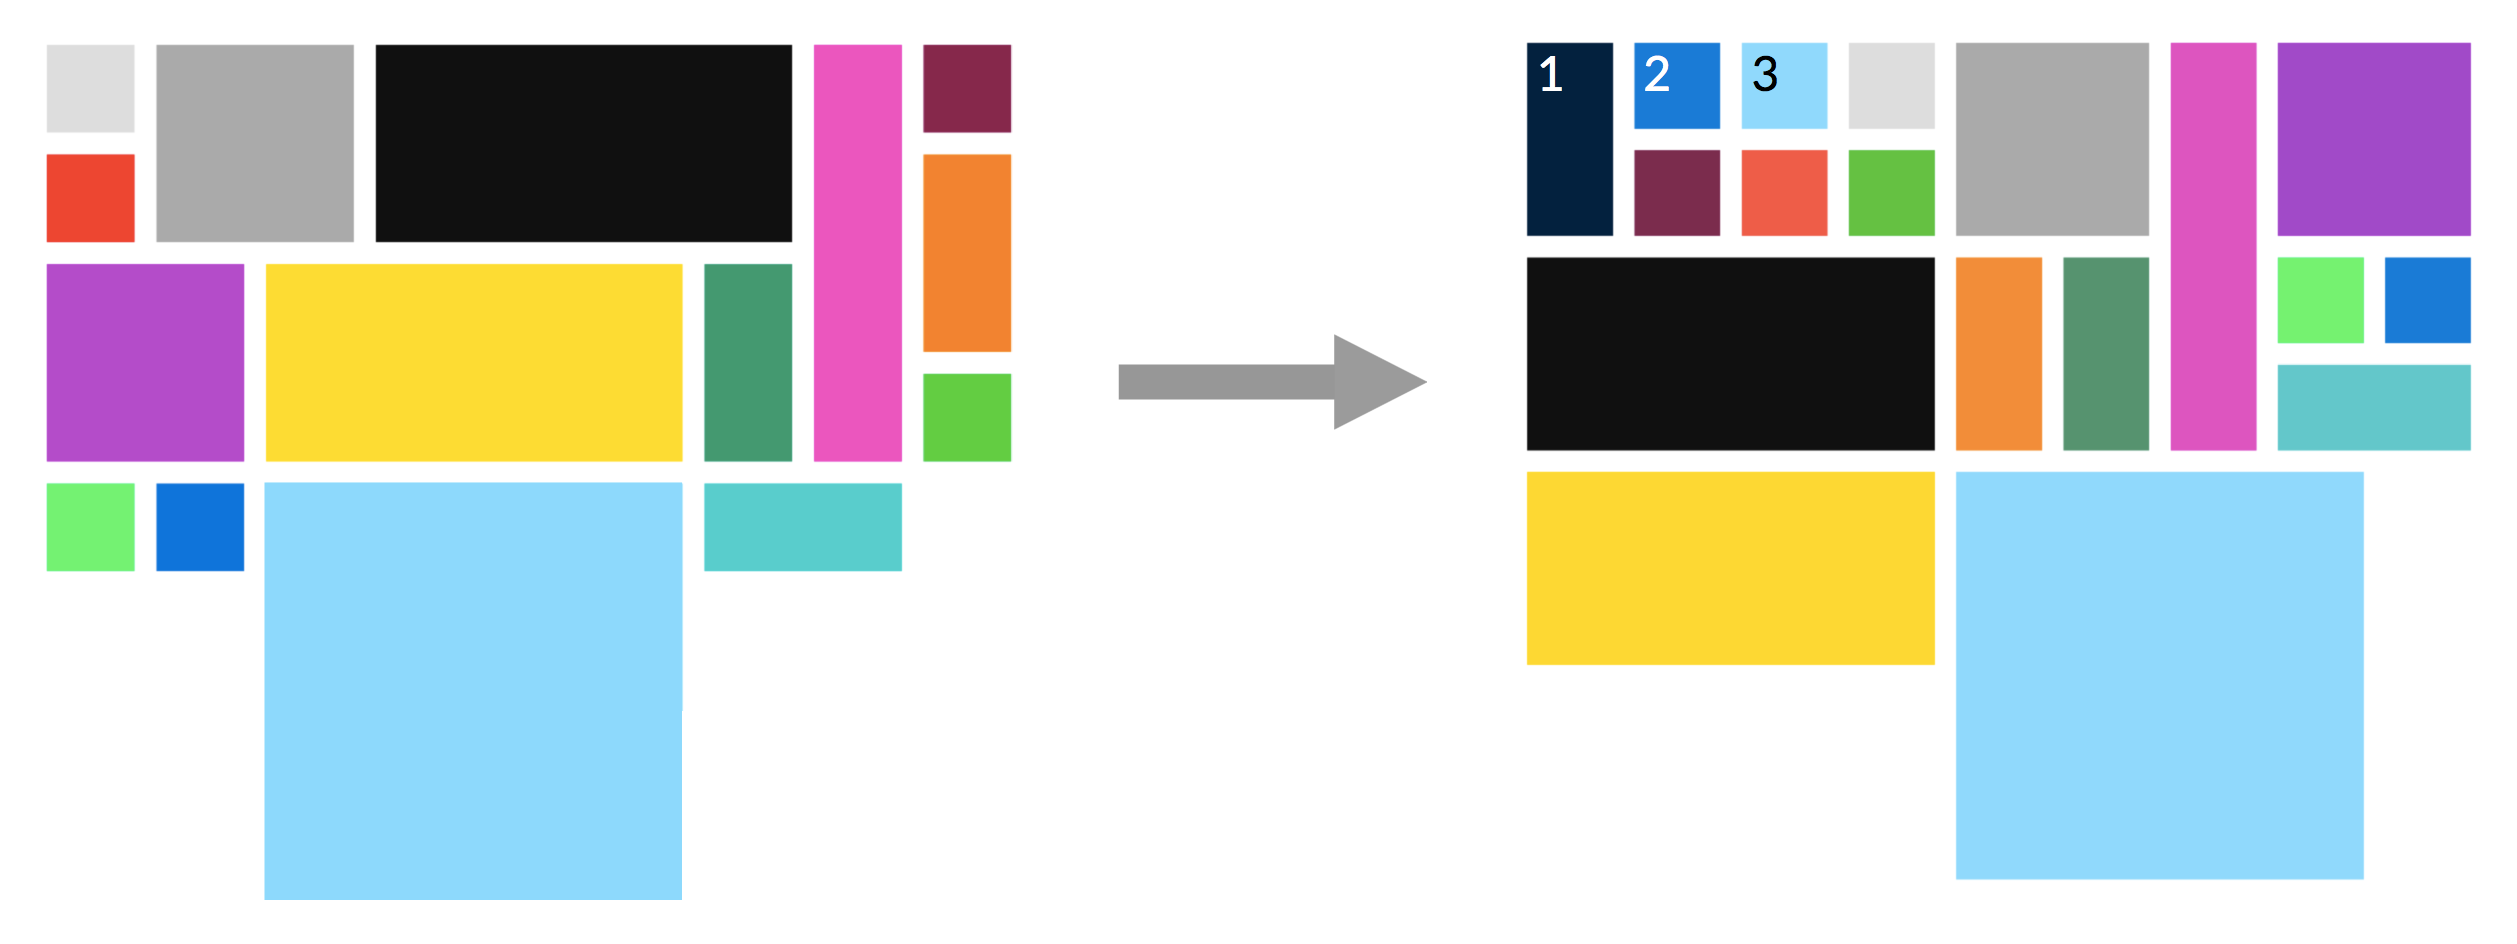
\includegraphics[width=0.8\textwidth]{images/grid_flow.png}
    \caption{Zu dem Grid links wurden die Elemente 1, 2 und 3 hinzugefügt. Das resultierende neue Layout ist rechts zu sehen. Dies ist ein praktisches Beispiel welches mithilfe von packery durchgeführt wurde.}
    \label{fig:grid_flow}
  \end{figure}


\subsection{Animationen}

Die Nutzung von funktionalen Animationen wurde in den letzten Jahren zu einem populären Mittel, um die Nutzererfahrung zu verbessern \cite{functionalanimations}. Vergleich hier zu Googles Material Design \cite{materialdesign}, bei dem eines der genannten Designziele ``Motion provides meaning'' ist. Bei diesem Design wird viel Wert darauf gelegt, mittels Animationen die Nutzererfahrung zu erhöhen. Genauer wird bei den Animationen geschrieben: ``In the world of material design, motion describes spatial relationships, functionality, and intention with beauty and fluidity'' (Google 2014, \cite{materialdesign}).
So war es auch hier eines der gesetzten Ziele, Animationen zu entwickeln, die, neben dem rein ästhetischen Aspekt, einen Vorteil im Verständnis des Datenflusses der Applikation ermöglichen.

\begin{enumerate}
  \item Neue Kacheln sollen von \textit{oben} kommen um einerseits zu zeigen, dass es neue Inhalte gibt, und andererseits um das vertraute Konzept zu benutzen, dass neue Dinge von oben kommen. Beispiele im echten Leben sind Börsenticker, Nachrichtenseiten oder die Abfahrttafeln an Bahnhöfen.

  \item Die neuen Kacheln ordnen sich an ihrem Platz ein, alte Kacheln machen dementsprechend Platz.
  \item Die Anzahl an Bewegungen soll minimal sein, um nicht unnötig vom eigentlichen Inhalt abzulenken.
\end{enumerate}

Nur das Spaltenbasierte Layout erfüllt diese Anforderungen für Animationen, da die Beispiele gezeigt haben, dass eine Neuberechnung des Layouts bei dem Kachelbasierten zu aufwändig ist, als dass nachverfolgt werden kann, wie die Kacheln sich bewegen, und welchen Gesetzmäßigkeiten sie unterliegen.

\subsection{Kacheln}\label{sec:tiles}

Das Design der Kacheln ist neben ihrer Anordnung die wichtigste Design-Entscheidung. Zusätzlich zu dem rein funktionalen Aspekt ist auch das Aussehen wichtig, da gewährleistet sein muss, dass Inhalte leicht voneinander unterschieden werden können und die Fülle an Information den Benutzer nicht überfordert.

Rein funktional besitzt eine Kachel folgende Funktionalitäten:

\begin{itemize}
  \item Anzeige des Inhalts und Möglichkeit diesen zu öffnen. Die Anzeige des Inhalts kann variieren.
  \item Benutzer können den Inhalt favorisieren (speichern) und bewerten.
  \item Es werden Metainformationen wie der Typ des Inhalts (PDF, Kontakt, etc) angezeigt.
  \item Kacheln können schnell zu dem Thema zugeordnet werden, dem sie assoziiert sind.
  \item Anzeige der letzten Interaktion mit der Komponente, um den sozialen Aspekt der Anwendung zu verdeutlichen.
\end{itemize}

Obwohl die Kacheln je nach dargestellten Inhalt stark variieren können, ist es ratsam ein einheitliches Benutzerinterface für die Interaktionen zu bieten. Auch sollten die Metainformationen gleich angezeigt werden.
Mit diesen Anforderungen kann eine funktionale Kachel konzipiert werden, siehe Abbildung \ref{fig:tile_prototype}.

\begin{figure}[htbp]
    \centering
    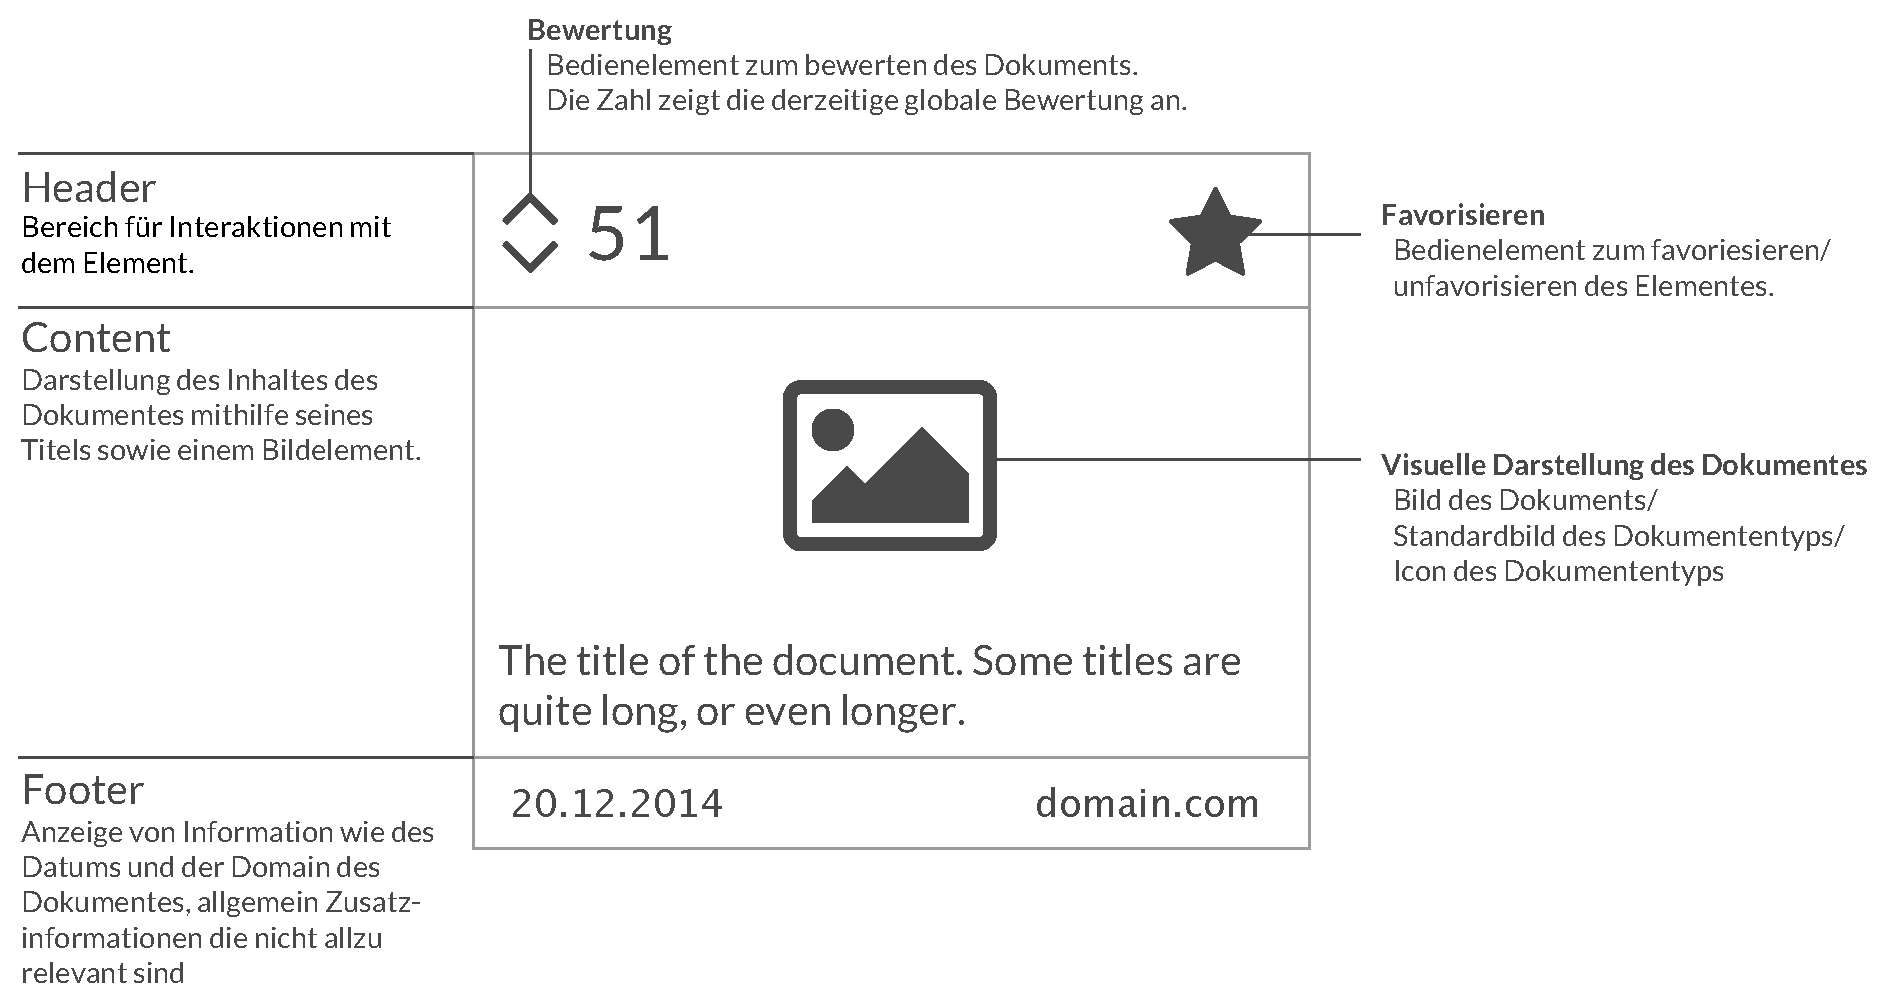
\includegraphics[width=1.0\textwidth]{images/tiles.eps}
    \caption{Ein Wireframe mit rein funktionalen Aspekten.}
    \label{fig:tile_prototype}
\end{figure}

Im Normalbetrieb des Infoboards werden gleichzeitig die Informationen mehrerer Themen angezeigt. Um diese Informationsfülle für den Benutzer verständlicher zu machen, sollte es für den Benutzer möglich sein, schnell zu sehen, welche Informationen zu welchem Thema gehören.
Menschen sind äußerst gut darin, Farben und unterschiedliche Formen schnell zu gruppieren. Nach aktuellem Kenntnisstand sind dies Teile der ersten Verarbeitungsstufe von visuellen Informationen \citep{treisman1987merkmale}. Eine schnelle Assoziation von Thema und Kachel ist elementar wichtig, deswegen wird die Hintergrundfarbe der Kachel dafür benutzt. Dies schränkt das Design aber insofern ein, dass bis auf Grautöne und Abstufungen der verwendeten Hintergrundfarbe keine anderen Farben mehr möglich sind. Man könnte zum Beispiel das Symbol zum Favorisieren nicht überall rot anzeigen. Doch war das dadurch erzielte Design so überzeugend, dass dies in Kauf genommen wurde. Ein erstes Design kann in Abbildung \ref{fig:tile_design} betrachtet werden.

\begin{figure}[htbp]
    \centering
    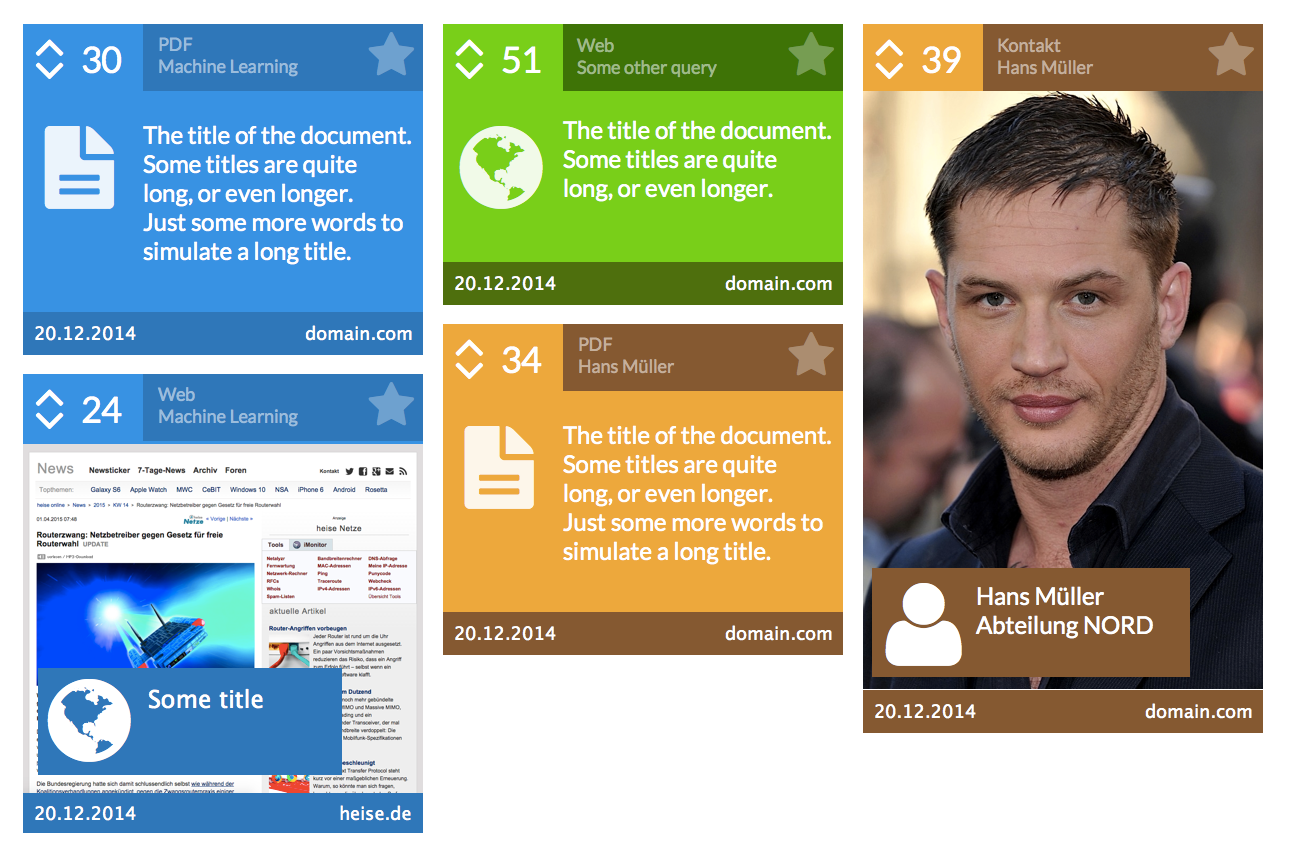
\includegraphics[width=1.0\textwidth]{images/tiles_real.eps}
    \caption{Ein erstes Design, dass verschiedene Darstellungsformen für unterschiedliche Typen von Informationen benutzt.}
    \label{fig:tile_design}
\end{figure}

\subsection{Eindeutige Zuordnung von Farben zu Themen}


Da in Abschnitt \ref{sec:tiles} entschieden wurde, die Hintergrundfarbe der Kacheln als Hauptunterscheidungsmerkmal der Themen zu verwenden, muss nun festgelegt werden wie eine Farbe zu einem Thema ausgewählt werden soll.
Es wird eine eindeutige Zuordnung von Farbe zu Thema benutzt, damit der Benutzer bei wiederholt gesuchten Themen, allein die Farbe benutzen kann um zu wissen, welches Thema eine Kachel hat.
Alle angezeigten Farben sollen optisch zueinander gehören und miteinander harmonieren. Um das zu erreichen, gibt es verschiedene Ansätze. Bei allen ist die Konvertierung des Themas zu einer Zahl, der \textit{erste} Schritt. Diese Funktion sollte die typischen Eigenschaften einer \textit{guten} Hash-Funktion mitbringen: gleichmässige Verteilung der Funktionswerte auf den Zielraum, minimale Kollisionen und Determinismus.
Die hier Verwendete stammt von Dan Bernstein und ist bekannt unter der Bezeichnung djb2 \cite{djb2}.

Der erste Ansatz wäre es, eine Liste mit zueinander harmonierenden Farben zu verwenden und jeweils eine auszusuchen. Das kann jedoch nur mit einer langen Liste von Farben funktionieren. Außerdem kann es bei dieser Methode häufiger vorkommen, das Themen dieselbe Farbe zugewiesen bekommen, was äußerst unerwünscht ist. Man könnte sich nun überlegen, ob komplexe Konfliktresolution, also wenn Themen miteinander kollidieren und einer davon eine andere Farbe bekommt, betrieben werden sollte.
Dadurch wird aber verhindert, dass jedes Thema konsistent die gleiche Farbe bekommt.

%TODO der satz mit naiv ist doof

Der zweite Ansatz besteht darin, die Farben prozedural zu erstellen.
Der naivste Ansatz wäre es hierbei den Wertebereich der Hash-Funktion auf $0 - 2^{16}$ einzuschränken, das Ergebnis in Hexadezimal umzurechnen und als RGB-Farbe zu benutzen. Die dadurch entstehenden Farben sind jedoch zufällig und würden nur per Zufall harmonieren. Ein weiteres Problem ist, das zu viele dunkle und helle Farben erstellt werden.

Der RGB-Farbraum ist nicht dazu geeignet die Helligkeit der entstehenden Farben zu kontrollieren, dafür sind Wahrnehmungsorientierte Modelle, die Farben durch Helligkeit, Sättigung und Farbton beschreiben, deutlich geeigneter \cite{meier2004interactive}. Die populärsten Wahrnehmungsorientierten Modelle sind die HSx-Räume wie HSV oder HSL.
Probleme von den HSx Farbräumen sind die für den Menschen ungünstige Verteilung der Farben und die Helligkeit der Farben, die bei Änderung des Farbtons stark varriert \cite{husl}.
Abhilfe schaffen die dafür erstellten Farbräume Lab (CIELAB) bzw. die Weiterentwicklung HCL (CIELUV). Sie sind jedoch nicht einfach zu benutzen, weil der valide Wertebereich der Eingabeparameter je nach Kombination der Werte unterschiedlich ist. Das macht es schwer, mit diesen Farbräumen Farben prozedural zu erstellen.
% Es gibt im speziellen um den Chroma-Wert, dieser kann grob mit der Helligkeit verglichen werden. Der Wertebereich der Sättigung und des Farbtons sind vom Chroma-Wert abhängig.

Die Wahl eines idealen Farbraums ist damit nicht eindeutig möglich, mittels der HSx-Räume ist es einfach, eine gute Farbskala prozedural zu erstellen, der Farbbereich ist jedoch ungünstig für den Menschen. LAB und HCL bieten die beste Farbverteilung für die menschliche Wahrnehmung, sind jedoch schwierig einzurichten. Eine mögliche Kombination der Vorteile beider Farbräume zeigt \citep{husl}. Hier wird ein Farbraum mit der Bezeichnung \textit{human-friendly HSL} (kurz HUSL) vorgestellt. HUSL bietet einen einfach zu bedienenden Farbraum, welcher versucht die Helligkeitsschwankungen bei Farbtonänderung zu minimieren und die Farbverteilung für das menschliche Auge zu optimieren.

Doch keiner der Farbräume konnte eine \textit{ideale} Farbskala erstellen. Es konnten in allen Farbräumen sehr anspruchsvolle Farbskalen mit wenig Kollisionen erstellt werden. Da Farbskalen ein subjektives Thema sind, wurde die Möglichkeit eingebaut, sie in der Applikation zu verändern - dies wurde gleich mit dem Gamification-Aspekt verbunden, wodurch man nach und nach neue Farbskalen Freischalten kann und der Nutzer sich diejenigen aussuchen kann, die ihm am meisten zusagen.

Zum Testen der Farbskalen wurde eine Liste von möglichen Themen benutzt. Die Ergebnisse sind in Abbildung \ref{fig:colors} zu sehen.

\begin{figure}[htbp]
    \centering
    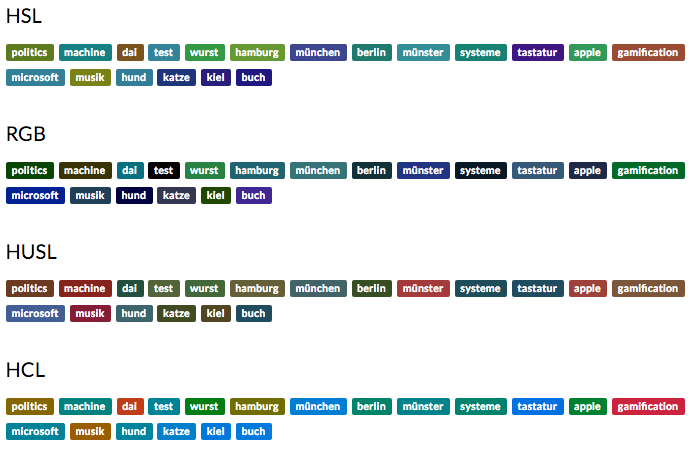
\includegraphics[width=1.0\textwidth]{images/colors}
    \caption{Farbskalen, die mit verschiedenen Farbräumen erstellt wurden.}
    \label{fig:colors}
\end{figure}

\section{Gamification}\label{chap:game}

% Es ist schwer neue Technologien im Unternehmensfeld einzuführen, vor allem wenn sie freiwillig benutzt werden können - so wie das hier entwickelte Enterprise Infoboard. Ziel ist es also durch die Gamification der Benutzung die Benutzer dazu zu motivieren die Anwendung gewohnheitsmäßig zu benutzen.

In Abschnitt \ref{sec:intro_game} wurde Gamification definiert, sowie anhand von Anwendungen gezeigt, dass Gamification einen Mehrwert für das Infoboard erzeugen kann. Im Folgenden werden die für das Infoboard eingesetzten Gamification-Mechanismen erläutert.

Die Grundlage unseres Spieledesigns ist der \textit{Compulsion Loop}, der ``eine modellierte Kette an Aktivitäten darstellt, die gewohnheitsmäßig wiederholt werden, um eine neurochemische Belohnung zu erhalten'' (\cite{gamasutra}, übersetzt aus dem Englischen)..

Nach \citep{gamasutra} besteht diese modellierte Kette aus 3 Schritten:

\begin{enumerate}
  \item \textbf{Anerkennung der Leistung} \\
  Die Ausführung der Aktionen wird belohnt, der Benutzer bekommt etwas das einen Wert für ihn besitzt. Die Herausforderung hierbei ist, etwas zu erschaffen, dass der Benutzer möchte und die Belohnung so einzuteilen, dass er gerade soviel bekommt, dass es eine Belohnung darstellt. Am Beispiel des Rollenspieles wäre eine Belohnung die verbesserte Rüstung, mit der der gespielte Charakter widerstandsfähiger wird und neue, bisher verschlossene Abenteuer bestreiten kann.
  \item \textbf{Belohnung einer Aktion}\\
  Jede Aktion, die der Benutzer ausführt, hat eine direkte Belohnung zur Folge. Diese ist jedoch zu gering, um sofortige Glücksgefühle auszulösen. Erst die  Anhäufung vieler Belohnungen führt dazu, dass der Benutzer die eigentliche \textbf{Belohnung der Leistung} erhält. Es ist zu beachten, dass diese direkten Belohnungen nicht allzu schnell die Möglichkeit freischalten, sie gegen dass einzutauschen wonach der Benutzer strebt. Im Rollenspiel könnte das Gold sein, dass benötigt wird um eine neue Rüstung zu kaufen.
  \item \textbf{Aktion}\\
  Die Aktion ist die Grundlage der Schleife. Aktionen sind das was der Benutzer ausführen soll. Im Rollenspiel könnte dies das Lösen von Aufträgen sein.
\end{enumerate}

Im Folgenden wird die Gamification des Infoboard anhand dieser Schritten modelliert.

\subsection{Aktionen und deren Belohnung}

Das Infoboard besitzt ausgewählte Interaktionsmöglichkeiten, die alle Teil der Aktionen sind, die eine Belohnung geben:

\begin{itemize}
  \item Bewertung der Suchergebnisse
  \item Favorisieren von Suchergebnissen
  \item Eingabe und Löschung von Themen
  \item Anmeldung und Abmeldung
\end{itemize}

Durch einige dieser Aktionen bekommt der Benutzer Punkte. Wichtig für uns ist es, dass die Bewertung der Suchergebnisse besonders gefördert wird, weswegen für diese Aktionen eine größere Punktzahl im Vergleich zu den anderen Aktionen vergeben wird.

\subsection{Anerkennung der Leistung}

Die Leistung des Benutzers muss anerkannt werden. Im Folgenden werden verschiedene Ansätze für Punkte, Bestenlisten und Abzeichen analysiert. Anhand dieser wird abschließend ein passendes Konzept für das Infoboard entwickelt.

\subsubsection*{Punkte}

Punkte sind unerlässlich im Spielekontext. Auch wenn die Punkte für den Benutzer nicht sichtbar gemacht werden, sind sie wichtig um dem Spieledesigner die Möglichkeit zu geben, das System zu evaluieren und daraufhin zu verändern \citep[pp. 36]{zichermann2011gamification}. Nach Zicherman \cite{zichermann2011gamification} unterscheidet man erhaltene Punkte in folgende Kategorien:

\begin{itemize}
	\item Erfahrungspunkte
    \item Eintauschbare Punkte
    \item Fähigkeitspunkte
    \item Karmapunkte
    \item Ansehenspunkte
\end{itemize}

Anstelle eines komplexen Spielesystems, wo verschiedene Punktesysteme benutzt werden, wurde hier entschieden, nur eine Art von Punkten zu benutzen, welche größtenteils auf den Erfahrungspunkten aufbauen.

Erfahrungspunkte stellen die wichtigste Kategorie von Punkten dar, jede Interaktion des Benutzers wird mittels Erfahrungspunkten festgehalten \citep[38 - 39]{zichermann2011gamification} und stellen bei einer bedachten Punktevergabe  eine gute Quantifizierung der Leistung des Benutzers da. Dadurch kann man Erfahrungspunkte gleichzeitig für eine Bestenliste benutzen - und damit als eine Art Ansehenspunkte. Um den Punktemechanismus noch etwas spannender zu gestalten, wurde Entschieden, dass sie gegen \textit{Booster} eingetauscht werden können. Mittels Boostern wird jeder Erhalt von Punkten für einen gewissen Zeitraum mit einem Multiplikator erhöht. So kann eine Kategorie von Boostern bewirken, dass der Benutzer für einen Tag die doppelte Anzahl an Punkten erhält.

Die Idee hinter den Boostern ist es, den Compulsion-Loop daraufhin zu unterstützen, dass der Nutzer sie kaufen wird, um seine Punktzahl noch weiter zu erhöhen. Durch die kurze Verweildauer des Boosters und dem Ziel des Benutzers seine Punkte zu erhöhen, wird dieser zwangsläufig seine Nutzung mit dem System erhöhen, da sich der Booster sonst nicht gelohnt hätte.

Die Punkte sind für den Benutzer immer sichtbar und aktualisieren sich in Echtzeit, sobald der Benutzer eine Aktion ausführt, die Punkte bringt. Zudem werden sie auf der Abzeichenseite nochmals dargestellt, wobei ein Balkendiagramm eine Kategorisierung anzeigt, wie der Benutzer diese Punkte genau erlangt hat, siehe Abbildung \ref{fig:points}.

\begin{figure}[htbp]
    \centering
    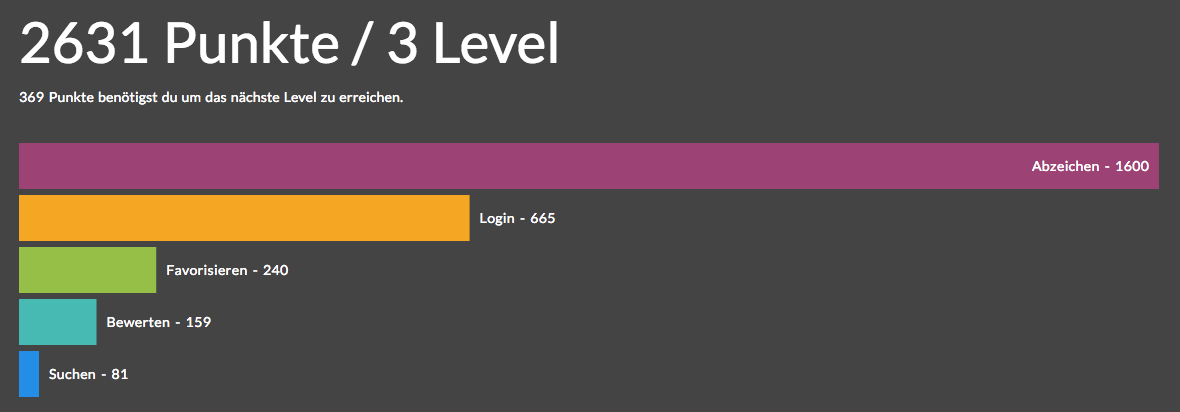
\includegraphics[width=1.0\textwidth]{images/infoboard_userstats.png}
    \caption{Die Punkte des Benutzers aufgeteilt in Kategorien.}
    \label{fig:points}
\end{figure}

Zusammengefasst benutzen wir \textbf{Erfahrungspunkte}, die für alle Aktionen vergeben werden und für \textit{Booster} ausgegeben werden können. Bestenlisten ermöglichen einen Vergleich der Punkte mit anderen Benutzern.

\subsubsection*{Bestenliste}

Damit der Benutzer sich mit anderen Vergleichen kann, werden Bestenlisten benutzt. Nach \citep[pp. 49 - 50]{zichermann2011gamification} sind Bestenlisten zu einem integralen Bestandteil unseres alltäglichen Lebens geworden. So sehr, dass wir sofort eine erkennen, wenn wir sie sehen. Beispiele für Bestenlisten im echten Leben umfassen die Ergebnisse der Stiftung Warentest, Klausurnotenhaushänge oder die Bundesligatabellen.

Nach \citep[pp. 50 - 51]{zichermann2011gamification} kann zwischen zwei Arten von Bestenlisten unterschieden werden, die \textit{lass-dich-nicht-entmutigen} und die \textit{unendliche} Bestenliste. Bei ersterer wird der Benutzer, egal welchen Platz er in der Bestenliste inne hat, immer direkt in der Mitte angezeigt. Hierbei ist es irrelevant ob er Platz 43 oder 40000 ist, er sieht sich selbst immer in der Mitte der Liste. Um sich herum sieht er seine direkte Konkurrenz. Wenn der Benutzer auf einen der Top 10/20/30 Plätze kommt, sollte sich dieses Verhalten jedoch ändern und er sollte die \textit{korrekte} Liste sehen.
Bei der \textit{unendlichen} Bestenliste werden alle Benutzer angezeigt, es gibt jedoch meistens die Möglichkeit die Anzahl der Benutzer zu verringern, so hat z.B. das Spiel Doodle Jump 3 Arten des Leaderboards: Lokal, Freunde und Global \citep[pp. 51]{zichermann2011gamification}.

Ein weiterer Aspekt ist der Zeitraum, der angezeigt wird. Vor allem bei Applikationen bei denen die Punktzahl immer weiter akkumuliert werden kann, und demnach unendlich viele Punkte zulassen, kann eine Bestenliste, die auf dem kompletten verfügbaren Zeitraum aufbaut, für Neuanfänger entmutigend wirken, da sie es wohl nie schaffen werden einen höheren Platz zu erreichen, wenn jeder doch gleich viele Punkte pro Tag erzielen kann.
Eine offensichtliche Lösung wäre es, den Zeitraum zu beschränken, zum Beispiel auf die letzen 7 Tage. Dies hat dann aber einen ähnlich negativen Effekt auf die dauerhaften Nutzer: Sie können ihre Vormachtstellung nicht demonstrieren.

Es wurde deswegen entschieden immer 2 Bestenlisten anzuzeigen: Eine mit dem kompletten Zeitraum und eine mit den letzten 30 Tage. Dadurch ist es möglich beide Parteien zufriedenzustellen, ohne Kompromisse eingehen zu müssen. Es werden ebenfalls beide Arten der Bestenliste benutzt: Im persönlichen Dashboard wird die \textit{lass-dich-nicht-entmutigen}-Bestenliste und in den globalen Statistiken wird eine \textit{unendliche} Bestenliste benutzt. Siehe Abbildung \ref{fig:leaderboarduser} für die \textit{lass-dich-nicht-entmutigen}-Bestenliste.

\begin{figure}[htbp]
    \centering
    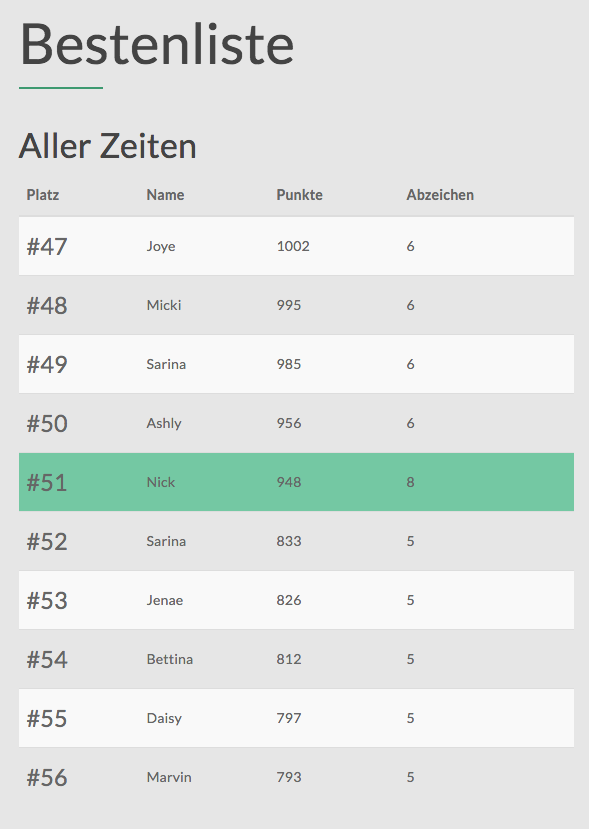
\includegraphics[width=0.8\textwidth]{images/infoboard_leaderboard_user.png}
    \caption{Die Benutzerzentrische \textit{lass-dich-nicht-entmutigen} Bestenliste, hier sieht sich der Benutzer immer in der Mitte der Liste.}
    \label{fig:leaderboarduser}
\end{figure}

\subsection{Abzeichen}
Abzeichen bzw. Badges sind ein etabliertes Element der Gamification. Nach \citep[pp. 55]{zichermann2011gamification} nutzen sie zahlreiche Eigenschaften der menschlichen Psyche, um begehrenswert zu sein: das menschliche Sammelverhalten, die plötzliche (positive) Überraschung wenn ein unerwartetes Abzeichen erhalten wurde, Sozialer Status (ähnlich zu Punkten), pure Ästhetik der Abzeichen und das Aufgabenziel, das hinter jedem Abzeichen steckt.

In manchen Fällen sind Abzeichen so effektiv eingesetzt, dass sie sogar Level mit speziellen Abzeichen ersetzen, als Beispiel sei Foursquare gennant, bei der der Benutzer das Abzeichen für das Erreichen einer bestimmten Anzahl an \textit{check-ins}\footnote{Der Begriff \textit{check-in} wird von vielen sozialen Diensten benutzt um an sich an einem realen Ort ``einzuchecken'' - um dies z.B. seinen Freunden mitzuteilen} erhält. Dies funktioniert bei Foursquare deswegen gut, weil \textit{check-ins} der wichtigste Bestandteil der Applikation sind \citep[pp. 57]{zichermann2011gamification}. Auch haben \textit{check-ins} keine negative Konnotation, da es zumeist als überaus positiv angesehen wird, wenn man häufig ausgeht und neue Orte erkundet.

Trotz aller positiven Aspekte von Abzeichen sind sie nicht einfach zu verwenden, so benutzt \citep[pp. 56]{zichermann2011gamification} den Begriff ``badgenfreude'' für ein Konzept, bei dem zu viele langweilige und sinnlose Abzeichen den Sinn von Abzeichen zunichte machen und sogar negative Folgen für das \textit{User Engagement} haben können.

Es ist sehr wichtig, dass die Abzeichen den Benutzer nicht stören. Er soll es mögen, sie zu bekommen. Aber wann mag er es Abzeichen zu bekommen, und wann stören sie?
Zunächst kann die Frequenz des Erhalts betrachten werden. Um anfangs den Benutzer zu motivieren gibt man ihm in der ersten Zeit meistens relativ viele Abzeichen, so ist es typisch ein Abzeichen für die erste Anmeldung oder die erste geschaffte Herausforderung zu geben.
Die Frequenz muss mit der Zeit nachlassen, damit sie den Benutzer nicht von der eigentlichen Applikation ablenken, und damit die Abzeichen weiterhin als wertvoll anerkannt werden.
Es sollte für den Benutzer immer offensichtlich sein wofür, er ein Abzeichen bekommen hat und welchen Wert es besitzt. Der Wert des Abzeichens sollte graphisch repräsentiert werden, zum Beispiel werden sehr oft die Farben Bronze/Silber/Gold als Analogie zu Medaillen benutzt, um den Wert zu symbolisieren.
Damit der Benutzer weiß, welche Abzeichen es noch gibt, und wie er sie erhalten kann, sollte es möglich sein, alle erhältlichen Abzeichen mit einer jeweiligen Beschreibung, wie man es denn erhält, einzusehen.

\begin{figure}[htbp]
    \centering
    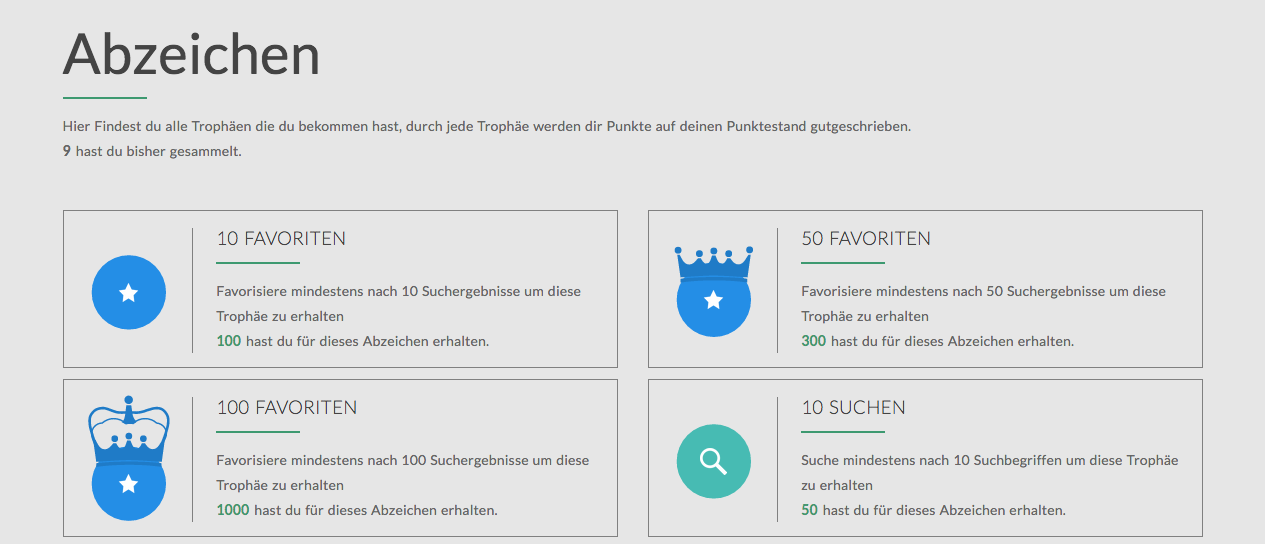
\includegraphics[width=1.0\textwidth]{images/infoboard_badges.png}
    \caption{Die Benutzeransicht für die erhaltenen Abzeichen. Der hier gezeigte Benutzer besitzt die Favoriten-Abzeichen in allen Ausführungen.}
    \label{fig:badges}
\end{figure}

So hat sich schlussendlich folgendes Schema für die Abzeichen des Infoboards ergeben. Es gibt 3 Kategorien von Abzeichen, die jeweils einen anderen Wert darstellen. Die erste Kategorie sind leicht zu erhaltene Abzeichen, die zweite sind mittelmäßig schwer zu erhaltene Abzeichen, d.h. der Benutzer es haben möchte, kann dieser es auch in angemessener Zeit erhalten. Die Abzeichen der letzten Kategorie benötigen ca. 50x mehr Zeit als die der ersten. Dadurch sollen auch Vielbenutzer weiterhin durch das System motiviert werden. Visuell wird der Wert durch eine Krone dargestellt, wobei die der letzten Kategorie am imposantesten aussieht, siehe dazu Abbildung \ref{fig:badges}.
Der Erhalt von neuen Abzeichen wird so schnell wie möglich dem Benutzer mitgeteilt - jede vom Benutzer ausgeführte Aktion wird an das Backend gesendet, welches \textbf{immer} berechnet, ob dieser dafür ein neues Abzeichen bekommt. Ist dies der Fall, wird das dem Frontend mitgeteilt und der Benutzer bekommt eine Nachricht angezeigt, siehe Abbildung \ref{fig:flashmessage}. Dieser Vorgang dauert weniger als eine halbe Sekunde.
Damit das Abzeichensammeln nicht langweilig und obsolet wird, sollten regelmäßig Neue eingeführt werden. Der Quelltext wurde daraufhin optimiert, dass dies keinen größeren Aufwand darstellt.

\begin{figure}[htbp]
    \centering
    
\includegraphics[width=0.8\textwidth]{images/infoboard_flashmessage.png}
    \caption{Um den Benutzer über das Erreichen eines neuen Levels oder den Erhalt eines Abzeichens zu informieren, werden Flashmessages benutzt.}
    \label{fig:flashmessage}
\end{figure}

\chapter{Technische Umsetzung}\label{chap:tech}

In Kapitel \ref{chap:concept} wurde die Applikation soweit geplant, dass die technische Umsetzung erfolgen kann. Viel Wert wurde darauf gelegt, die getroffenen Technologieentscheidungen, wie auch die gewählte Architektur, zu begründen.
Die technische Umsetzung wird sich größtenteils mit dem Frontend beschäftigen, das Backend wird kurz in Kapitel \ref{sec:backend} behandelt.


\section{Wahl der Technologie}

Die erste Frage die sich bei der Umsetzung stellt, ist welche Technologie verwendet werden soll.

Die Wahl derer ist ein wichtiger Punkt, der die darauffolgende Entwicklung und spätere Wartung beeinflusst \cite{graham2004beating}. Es wird versucht auf folgende Punkte einzugehen:

\begin{itemize}
  \item Die Technologie ist \textit{erwachsen} \\
  Die verwendete Bibliothek oder ähnliches ist nicht allzu neu und hat sich in vielen Applikationen bewährt. Sie ist soweit ausgereift, dass Umgehungslösungen oder Fehlerbehebungen nur in den seltensten Fällen nötig sein sollten.
  \item Die Technologie hat keine große Einstiegsbarriere \\
  Es wird versucht, nicht allzu viele Frameworks zu benutzen und wenn, dann welche, die weitestgehend bekannt sind, und/oder in dem DAI-Labor viel benutzt werden. Wenn Bibliotheken verwendet werden, wird darauf geachtet, dass sie einfach zu lernen sind und intuitiv in der Benutzung sind.
  \item Die Technologie ist zukunftssicher \\
  Es ist immer schwer abzuschätzen, welche Technologie länger überleben wird, doch wird versucht anhand von Faktoren wie Popularität, Aktivität der Entwicklung und Einsatz bei großen Firmen, dies so gut wie möglich zu garantieren.
\end{itemize}

\subsection{Programmiersprache}

Die wichtigste Wahl ist die Wahl der Programmiersprache \cite{graham2004beating}. Im Frontend wird diese Entscheidung größtenteils dadurch abgenommen, dass aktuelle Browser exklusiv die Ausführung von JavaScript beherrschen, andere Sprachen sind nur über Erweiterungen (Flash, Java, Silverlight) verfügbar, deren Relevanz in den letzten Jahrzehnten soweit abgenommen hat, dass sie für uns keine Option mehr darstellen \cite{clientside}.

JavaScript ist allerdings nicht die beliebteste Sprache. Die Tatsache das die Sprache in ca. 10 Tagen geschrieben wurde mag dazu beigetragen haben \citep{severance2012javascript}. So kam es, dass JavaScript in den letzten Jahren immer mehr zu einem Kompilierungsziel geworden ist, d.h. andere Programmiersprachen kompilieren zu validem JavaScript-Quelltext. Diese Praxis ist mittlerweile so populär geworden, dass JavaScript auch als \textit{Assembly of the Web} bezeichnet wird \cite{webassembly}. Die populärsten Programmiersprachen, die zu JavaScript kompilieren, sind vermutlich CoffeeScript, TypeScript und Java (mittels GWT). Die Liste der Sprachen ist endlos mit über 300-Sprachen, die zu JavaScript kompilieren. Eine Auflistung jener ist auf dem Github-repository von CoffeeScript zu finden \cite{javascriptcompile}.

Zakai \citep{zakai2011emscripten} veröffentlichten mit \textit{emscripten}, das mit Abstand aufwändigste Projekt in diesem Bereich. Dies ist ein LLVM-zu-JavaScript-Kompilierer, mit dem es unter anderem möglich ist C++-Quelltext zu JavaScript zu kompilieren, wodurch zum Beispiel der TeX-Compiler im Browser ausgeführt werden konnten \cite{texlive}.

Die Nutzung dieser Sprachen, vor allem der populärsten, hat viele Vorteile: von vereinfachter Syntax (CoffeeScript) bis hin zu statischer Typisierung (Google Web Toolkit - GWT). So bleibt die Frage, ob es überhaupt noch zukunftssicher bzw. praktikabel ist reines JavaScript zu benutzen.
Die Frage kann mit einem klaren Ja beantworten werden, wenn eine Prämisse an die Ausführungsumgebung gesetzt wird: Sie unterstützt JavaScript in der Version 6, bzw. ECMAScript 6 (Im nachfolgenden mit ESx abgekürzt).
Die für JavaScript zuständige Organisation ECMA investierte viel Arbeit, um die Tatsache, dass JavaScript nur in 10 Tagen geschrieben wurde, etwas weniger offensichtlich zu machen. Mit ECMAScript 6 \cite{es6} trägt diese Arbeit am deutlichsten Früchte. Funktionalitäten wie Destructuring, Generators , Modules, Template Strings oder Promises lassen ES6 zu einer modernen Sprache werden.

Die aktuellen Browser unterstützen bisher nur einen Bruchteil der ES6 Spezifikation, eine komplette Übersicht ist unter \cite{es6features} zu finden. Es gibt keine offizielle Stellungnahme seitens der Browser-Hersteller wann ES6 komplett unterstützt werden wird, doch kann davon ausgegangen werden, dass dies in den nächsten Jahren geschieht, wenn die ES5-Unterstützung als Vergleich benutzt wird. Etwa zwei Jahre nach offizieller Festlegung von ES5, unterstützten die populärsten Browser ES5 vollständig \cite{es5adoption}.

Doch sind die Vorteile so überwiegend im Vergleich zu ES5, dass eine Nutzung von ES6 äußerst wünschenswert ist.
Die Lösung des Problems wurde im Grunde schon erwähnt: Man kompiliert JavaScript zu JavaScript bzw. ES6 zu ES5.
Die Tatsache, dass JavaScript heutzutage immer im Zusammenhang mit Build-Tools benutzt wird, um zum Beispiel den Quelltext verkleinern oder ihn unlesbarer zu machen, bedeutet, dass der Entwickler nur minimalen Aufwand betreiben muss damit er ES6 auch in ES5 Umgebungen benutzen kann.

So wurde für diese Arbeit entschieden, dass ES6 die beste Wahl für die Programmiersprache ist. Alle Browser werden ES6 in Zukunft unterstützen, womit ES6 keinesfalls eine obsolete Sprache werden wird. Außerdem ist im Vergleich zu den richtigen Kompilier-zu-JavaScript-Sprachen ES6 die geringste Hürde für neue Entwickler, die JavaScript schon kennen: ES6 ist abwärtskompatibel und die neuen Funktionalitäten können in wenigen Stunden gelernt werden, wenn das überhaupt nötig ist.

Neben reinem ES6 benutzen wir jedoch auch noch eine von Facebook entwickelte Erweiterung namens JSX \cite{jsx}. Diese erweitert JavaScript mit der Möglichkeit, UI-Komponenten mit einer HTML-Syntax zu beschreiben. Dies wäre z.B. valides JSX:

\begin{minted}{text}
    var header = <h1>Überschrift</h1>;
\end{minted}

Die direkte Einbettung von HTML-Markup in JavaScript wird derzeit kontrovers diskutiert \cite{jsxcontrovers}, doch wird dadurch die Benutzung von der hier verwendeten Interface-Bibliothek React.js deutlich vereinfacht.
Bisher ist JSX ein Vorschlag von Facebook an ECMA, doch ist die Benutzung von JSX mittlerweile sehr verbreitet. So unterstützt eslint \cite{eslint} wie auch der ES6-ES5-Kompilierer Babel JSX \cite{babel}, dass eine Integration etwas JSX-ähnlichem ziemlich wahrscheinlich ist.
Mittels ES6-templatestrings ist es möglich \textit{Domain Specific Languages} zu schreiben, so gibt es mittlerweile auch ein proof-of-concept JSX rein in ES6 zu schreiben \cite{templatestrings}.

Neben Javascript, muss, um die Anwendung zu gestalten, CSS (Cascading Style Sheets) geschrieben werden. CSS besitzt einige Schwächen, deshalb versuchen Projekte wie less \cite{less} oder sass \cite{sass} diese zu beheben, indem sie CSS mit Funktionalitäten wie Variablen, Mixins und Verschachtelung erweitern.
Allgemein werden diese Projekte CSS-preprocessors gennant, und funktionieren,
ähnlich wie den Kompilier-Zu-JavaScript-Sprachen, indem sie die in ihrer Sprache geschrieben Dateien in CSS übersetzen \cite{csspre}.
Es hat sich bewährt less oder sass zu benutzen, da damit die Effizienz der Entwicklung gesteigert werden kann \cite{csspre}. So wurde auch für diese Applikation entschieden less zu benutzen, da damit auch Bootstrap geschrieben wurde - das hier verwendete CSS-Framework.
Das Ausmaß dieser Entscheidung ist jedoch kein Vergleich zu der Programmiersprachen-Entscheidung, weswegen es sich nicht lohnt, die Kosten/Nutzen genauer zu betrachten.

\subsection{Ladezeiten}\label{sec:loadingtimes}

Ein großer Faktor der in anderen Umgebungen schon lange keine Rolle mehr spielt, ist die Größe des Quelltextes. Bevor in JavaScript irgendeine Bibliothek benutzt werden kann, muss sie zuerst beim Benutzer heruntergeladen und ausgeführt werden, was bei langsamen Computern mit schlechter Internetverbindung einen großen Zeitaufwand bedeutet. Um den Punkt nochmal zu verdeutlichen, wurde ein kleiner Test durchgeführt. Dazu wurde eine EmberJS-Demoapplikation ausgeführt,\footnote{Auf einem Macbook Air mid 2013 in Minimalkonfiguration und dem Chrome Browser in Version 41, die vorhandene Internetverbindung hatte eine Übertragungsrate von $50000 \frac{\text{bit}}{s}$} die sehr wenig wirkliche Logik besitzt, sodass gut zu zeigen ist, wie viel das Herunterladen und Ausführen nur der Bibliotheken ausmachen.
Die Anwendung ist auf Github zu finden \cite{embercrud}.
\begin{figure}[htbp]
    \centering
    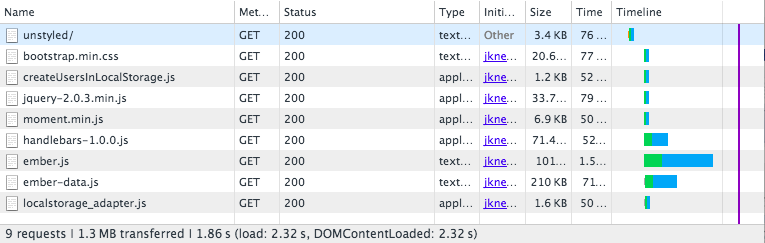
\includegraphics[width=0.8\textwidth]{images/performance_1.png}
    \caption{Übertragungszeit der benötigten Dateien}
    \label{fig:loadtimes}
\end{figure}
\begin{figure}[htbp]
    \centering
    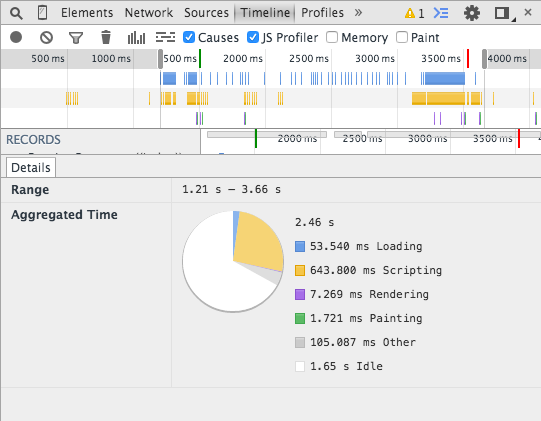
\includegraphics[width=0.6\textwidth]{images/performance_2.png}
    \caption{Benötigte Ausführungszeit der Skriptdatein}
    \label{fig:executiontime}
\end{figure}
Die Ergebnisse zeigen, dass ganze $1.86s$ zum Übertragen und etwa $600ms$ zum ausführen den Anwendung benötigt wurden.

Aufgrund dessen wurde, neben dem Versuch möglichst wenige Bibliotheken oder Frameworks zu benutzen (z.B. wenn nur eine Funktion einer großen Bibliothek benutzt wurde, wurde diese Funktion durch eine minimalere Bibliothek ersetzt oder selbst geschrieben bzw. kopiert), auch diverse Techniken zum Minimieren des Quelltextes genutzt.

\subsection{Frameworks und Bibliotheken}

Es wurden schon etliche Webanwendungen entwickelt, somit gibt es kaum ein Problem, das noch nicht gelöst wurde. Es gibt tausende JavaScript-Bibliotheken und Frameworks, die einem das Leben einfacher machen sollen. Ein klarer Platzhirsch ist jedoch nur für Subkategorien wie Datenvisualisierung zu finden.

Es ist schwer in der Welt der Webanwendungen mit der Geschwindigkeit, in der neue (und auch praktikable) Bibliotheken und Frameworks veröffentlicht werden, mitzuhalten. Der nachfolgende Abschnitt befasst sich deshalb ausführlicher mit der Entscheidungsfindung in diesem Bereich und zeigt auf, welche Aspekte alles beachtet werden müssen.

Die einflussreichste Entscheidung hierbei ist diejenige für ein Framework wie Dojo\cite{dojo}, AngularJS\cite{angularjs} oder EmberJS\cite{emberjs}.
Nach \cite{prosandcons} gibt viele Vorteile die für die Benutzung eines Frameworks sprechen: Große Benutzergemeinde, getestete Komponenten, Cross-Browser Unterstützung, eine immense Anzahl an vorgefertigten Lösungen für häufige Probleme/Aufgaben, eine klare Projektstruktur und viele vorgefertigte Komponenten.

Die Benutzung eines Frameworks spart also Zeit und beschleunigt die Entwicklung, doch gibt es auch Gründe, warum immer mehr Leute sich von den großen Frameworks abwenden \cite{nomoreframeworks, frameworkless}.
Alle Frameworks besitzen eine große Lernkurve, jeder Entwickler ist gezwungen, das Framework zu lernen, um produktiv mitzuarbeiten, da ein Framework jeden Aspekt der Anwendung berührt. Frameworks veralten schnell, und auch bei aktiver Entwicklung sind ständige API-Änderungen der Standard. Dem Entwickler bleibt nichts anderes übrig als sich mit dem Framework zu bewegen. Die vom Framework bereitgestellten Abstraktionen sind oft nicht optimal und verbergen zu viel, oder sind auf einen bestimmten Benutzungszweck hin optimiert, womit sie mehr ein Hindernis darstellen können, sobald etwas gemacht werden muss, das die Entwickler vergessen haben zu beachten.
Weiterhin ist jede vom Framework erschaffene Abstraktion mehr ausgeführter Quelltext, und wenn diese nicht gerade direkt der Geschwindigkeit der Applikation zu gute kommen, verlangsamen sie die Applikation. Dies ist normalerweise nicht so sonderlich wichtig, jedoch sind Webanwendungen Benutzerinterfaces, bei der die Geschwindigkeit einen erheblichen Teil der Benutzererfahrung ausmacht, siehe dazu auch Abschnitt \ref{sec:loadingtimes}, indem gezeigt wird, dass die Größe des Quelltextes einen erheblichen Einfluss auf Ladezeiten hat.

Allen Vorteilen zum Trotz wurde für diese Arbeit entschieden, dass die Benutzung eines Frameworks nicht die optimale Lösung ist, weil zum Beispiel die Visualisierung so aufwändig ist, dass unsere Erfahrung mit großen Frameworks es deutlich machten, dass die gegebenen Abstraktionen derer nicht ausreichen würden.

Es wurde deshalb entschieden eine Ansammlung von Bibliotheken zu benutzen, die sich für ihren Bereich bewährt haben. Dadurch wird garantiert, dass die bestmögliche Benutzererfahrung möglich ist, weil sobald eine Bibliothek nicht ausreicht, ersetzt oder ergänzt werden kann.

Es wurden am Ende folgende Bibliotheken verwendet

\begin{description}
	\item[React.js \cite{react}] wird für die komplette Darstellung der Applikation benutzt. Im nächsten Abschnitt wird auf React.js noch genauer eingegangen, da es viele Innovationen in diesen Bereich bringt.
	\item[react-router \cite{reactrouter}] ist eine routing-Bibliothek für react und macht es sehr einfach URLs zu einer View zuzuordnen.
	\item[refluxjs \cite{reflux}] ist eine Bibliothek für eine unidirektionelle-Datenfluss Architektur, mehr dazu im nächsten Abschnitt.
	\item[bootstrap \cite{bootstrap}] ist das meist benutzte CSS-Framkework und vereinfacht das Erstellen von responsiven Applikationen. Weiterhin stellt es einige nützliche Komponenten wie z.B. eine Navigationsleiste bereit.
	\item[react-bootstrap \cite{reactrouter}] bietet für alle verfügbaren bootstrap-Komponenten die entsprechenden react-Komponenten.
	\item[d3.js \cite{bostock2011d3}] ist die berühmteste Bibliothek für Visualisierungen. Hiermit wurde das animierte Säulendiagramm geschrieben, aber auch vieles der Farberzeugung entstand mithilfe von d3.js.
	\item[immutable.js \cite{Immutable}] bringt nicht veränderbare Datenstrukturen in die Welt von JavaScript. Sie wurde bei der Verarbeitung der Suchergebnisse bis hin zu deren Darstellung benutzt, der Vorteil wird unten noch genauer betrachtet.
	\item[lodash \cite{underscore}] ist eine utility-Bibliothek mit einem starken Fokus auf funktionaler Programmierung. Sie wurde so ziemlich überall in der Applikation benutzt.
	\item[cookies-js \cite{cookiesjs} / store.js \cite{storejs}]sind mini-Bibliotheken, die das Arbeiten mit \texttt{cookies} und \texttt{localstorage} vereinfachen. \texttt{cookies} werden benutzt, um den Benutzer eingeloggt zu lassen und \texttt{localstorage} um Suchergebnisse zu cachen.
	\item[moment.js \cite{momentjs}] vereinfacht den Umgang mit Datums-Objekten und bietet Funktionen wie \texttt{add(1, \'day\')} und erweiterte Formattierungsmöglichkeiten.
\end{description}

\subsection{Tooling}

Das Tooling im Frontend hat sich in den letzten Jahren rasant verändert, kaum jemand schreibt heutzutage noch JavaScript oder CSS, ohne dass ein sogenanntes Build-Tool diese Dateien nochmals verändert.

Die bekanntesten Build-Tools sind Gulp\cite{gulp}, Grunt\cite{grunt}, Webpack\cite{webpack} und Brunch\cite{brunch}.

Webpack stellt eine Ausnahme dar, da es im Grunde gar kein Build-Tool ist, sondern ein \textit{module bundler}, d.h. es verarbeitet alle in der Entwicklung relevanten JavaScript/CSS/Bild-Dateien und bündelt diese. Durch die Architektur von Webpack ist es möglich, so ziemlich jeden Datei-Typ zu verarbeiten.
Da die meisten Build-Systeme eben diese Ausgabe haben, kann Webpack die meisten Aufgaben von Build-Tools ersetzen.

Zwar ist Webpack noch ein junges Projekt, aber es hat sich schon für große Projekte wie Instagram bewährt \cite{petehuntwebpack}.

Für dieses Projekt viel die Wahl auf Webpack, weil es von allen Build-Tools die folgenden Dinge am besten realisieren konnte:

\begin{enumerate}
	\item Es muss möglich sein JavaScript-Bibliotheken mittels dem \texttt{npm}-Packetmanager zu benutzen.
	\item ES6-Quelltext muss zu ES5 Quelltext kompiliert und gebündelt werden.
	\item Wenn der Quelltext \textit{minified} wird, müssen SourceMaps erstellt werden.
	\item *.less-stylesheets müssen in CSS umgewandelt und gebündelt werden.
	\item Bei Dateiänderungen in der lokalen Entwicklungsumgebung sollte erneut kompiliert werden und die Seite aktualisiert werden.
\end{enumerate}

Die Konfigurationsdatei von Webpack dafür ist keine 50-Zeilen lang und einfach zu lesen\footnote{Die Datei befindet sich in \texttt{frontend/webpack.config.js}.}. Neben den aufgelisteten Anforderungen besitzt Webpack als einziges Build-Tool die Möglichkeit, bei Dateiänderungen, die Änderungen ohne Neuladen der Applikation einzufügen\footnote{hotmodule}. Durch den dadurch schnelleren Iterationszyklus, wird die Entwicklung beschleunigt. Dies allein ist eine so nützliche Funktionalität, dass Webpack  den anderen Möglichkeiten vorgezogen werden sollte.

\subsection{Facebook React und die Flux Architektur}\label{sec:flux}

Facebooks React.js ist eine JavaScript-Bibliothek, die seit ihrem erscheinen im Jahr 2013 viel Beifall geerntet hat. Zum Zeitpunkt dieser Arbeit wird sie produktiv von zahlreichen Firmen benutzt wie z.B. Khan Academy\cite{khan}, Netflix\cite{netflix} und AirBnB\cite{airbnb}. Facebook benutzt sie für seine größten Produkte: Facebook und Instagram (Google benutzt das hauseigene Framework AngularJS nicht für das Flagschiff Google Mail).

React.js ist jedoch kein Framework wie AngularJS oder Ember, es gibt keine Directives, Controllers, Templates oder Models. Das Einzige, was React.js bietet, sind Components, welche ähnlich wie der kommende Standard der \textit{Web Components} \cite{webcomponents} wiederverwendbare Interface-Widgets darstellen, indem Sie HTML/CSS und JavaScript koppeln und vom Rest des Systems separieren.

Dabei folgt React.js nicht den \textit{best-practices}, die in den letzten Jahren in Webentwicklung entstanden sind und sich in MVC-Frameworks widerspiegeln. Klassisch gibt es ein Template, das in HTML oder einer ähnlichen Sprache wie YAML geschrieben ist und Platzhalter enthält, die später gefüllt werden - dies ist das V in MVC.
Dazu kommt ein Controller, der diese Templates mit Daten füllt, auf welche Art ist nicht relevant. Kommuniziert der Controller mit einem Server, um Daten zu übertragen wie die eines Benutzers, stellt dies das M dar, also nicht die Kommunikation selbst, sondern die Datenstrukturen auf beiden Seiten, die den Benutzer darstellen.
Applikationen auf diese Weise zu erstellen, hat sich bewährt, was allerdings nicht heißt, dass es keine Kritik gibt.

\subsubsection*{Virtual DOM}

Einer der innovativsten Aspekte von React ist die virtuelle Repräsentation des DOMs (Document Object Model \cite{DOM}). Die normale Interaktion mit dem DOM ist langsam und kompliziert. Es ist schwer den aktuellen Status der Applikation darüber abzubilden - so geschieht das häufig über CSS-Klassen oder spezielle Attribute.
Eine Lösung dieses Problems ist es, die Applikation so zu schreiben, dass der ganze DOM bei jeder Veränderung des Zustands neu gerendert wird. (Vergleich hier zu Server-seitigem Rendern wo genau dies gemacht wird.) Natürlich wäre die Applikation bei so einem Vorgehen langsam (weil der Browser das rendern übernimmt) und Dinge, wie der Fokus auf Eingabe-Feldern, würde verloren gehen, was nicht besonders benutzerfreundlich wäre.

Mittels eines virtuellen DOMs kann dies deutlich effizienter und benutzerfreundlicher gestaltet werden. Bei jeder Zustandsänderung wird ein neuer virtueller DOM erstellt und mit dem alten virtuellen verglichen, wodurch die minimalen Änderungen erfasst werden können, um den derzeitigen DOM zum Zustand des Neuen zu überführen. Dies macht Frameworks, die einen virtuellen DOM benutzen deutlich schneller, als solche die die Hauptarbeit auf dem richtigen DOM verrichten. Das ganze Konzept ist im Gegensatz zu Technologien wie dem \textit{dirty checking} von AngularJS, welches eine Komplexität von $O(n^2)$ bis $O(n^{10})$ (Ab 10 Iterationen wird abgebrochen) besitzt, wobei $n$ die Anzahl der veränderbaren Inhalte ist \cite{dirty}, skalierbar.
Der von React.js verwendete Algorithmus besitzt eine Komplexität von $O(n)$, wobei $n$ die Anzahl der DOM-Elemente ist \cite{reactreconciliation}.
Ein Geschwindigkeitsvergleich von Frameworks, die einen virtuellen DOM benutzen, zeigt Abbildung \ref{fig:elm}, bei welcher die verschiedenen Frameworks anhand ihrer TodoMVC Implementierung verglichen werden.\footnote{Der TodoMVC ist ein Versuch die schiere Anzahl an Webframeworks anhand eines realen Beispiels zu vergleichen. Siehe \url{http://todomvc.com/}}.

\begin{figure}[htbp]
    \centering
    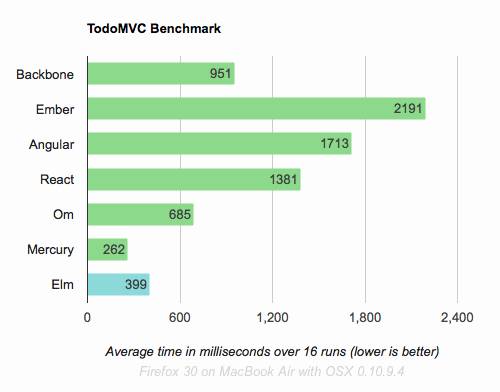
\includegraphics[width=1.0\textwidth]{images/virtual_dom.png}
    \caption{Geschwindigkeitsvergleich von TodoMVC-Implentierungen mit verschiedenen Frameworks \cite{elm}.}
    \label{fig:elm}
\end{figure}

Es ist zu sehen, dass Ember und AngularJS am langsamsten sind. Backbone ist in diesem Benchmark schneller als React.js, wobei die verwendete Implementierung der React.js-App nicht optimiert ist - Om\cite{om} kann als optimierte React-Version betrachtet werden, da Om im Grunde React.js mit nicht veränderbaren Datenstrukturen\footnote{Durch nicht veränderbare Datenstrukturen kann das diffing noch effizienter gestaltet werden, da viele Teilbäume nicht betrachtet werden müssen.} (immutable data-structures) ist. Mittels Backbone wie aber auch JQuery oder Dojo können theoretisch Applikationen geschrieben werden, die optimial in Geschwindigkeit sind. Dafür müsste der Programmierer bei jeder Zustandsänderung wissen, welche Teile des DOMs genau upgedatet werden müssen. Dieser Ansatz ist Erfahrungsmäßig nicht skalierbar, da bei solchen Optimierungen oft Grenzfälle vergessen werden und die Größe und Komplexität des Quelltextes stark zunimmt.

Die beiden schnellsten Frameworks, benutzen ebenso eine virtual-DOM Implementierung und wie Om, auch nicht veränderbare Datenstrukturen.
Dies ist auch der Grund, weswegen immutable.js\cite{Immutable} verwendet wurde, denn dies konnte die render-Geschwindigkeit in den aufwändigsten Teilen verbessern.

Ein weiterer Vorteil der virtuellen Darstellung ist die Unabhängigkeit des Browsers, um die Applikation zu rendern. Das schlussendliche Rendern des virtuellen DOMs in den richtigen DOM ist nicht zwingend. Es ist z.B. möglich, den virtuellen DOM in ein Canvas-Element zu rendern, oder in einen HTML-String zu konvertieren.
Durch das simple rendern zum HTML-String, was ganz ohne Browser möglich ist, beherrscht React.js isomorphes Rendering, d.h. Inhalte können auf dem Server und im Clienten gerendert werden. Erste Versuche zeigen, dass man dies komplett agnostisch machen kann und alles auf dem Server/Client gerendert werden kann, ohne dass der Benutzer einen Unterschied merkt \cite{overblog}. So ist es denkbar das schwache Geräte mehr auf dem Server rendern und somit komplexe Inhalte vergleichsweise schnell darstellen können.

\subsubsection*{Flux Architektur}

Flux ist die Applikations-Architektur, die Facebook für ihre Frontend-Applikationen benutzt. Es ergänzt React.js insoweit, dass es einen unidirektionalen Datenfluss ermöglicht \cite{flux}. Es ist wie eine Alternative zu MVC zu verstehen und ist eher ein Muster um Applikationen zu schreiben als ein Framework, das einem rigoros die Struktur vorschreibt. Im Allgemeinen benutzt Flux das Paradigma der Datenfluss Programmierung\cite{johnston2004advances}, bei der ein Programm als gerichteter Graph modelliert wird. Typisch für das Paradigma ist die Benutzung eines Beobachter-Entwursfmuster, wie eines pub/sub-System. Eine Auflistung und Bewertung typischer Muster ist unter \citep{signals} zu finden. Bei Flux wird für letzteres eine Abwandlung eines pub/sub-Systems benutzt.

Flux besitzt drei große Bestandteile: Einen Dispatcher, Stores und Views (React.js components). Des Weiteren gibt es Actions, sie sind Hilfsmethoden vom Dispatcher und werden benutzt, um eine semantische API zu unterstützen, die alle möglichen Veränderungen in der Applikation beschreibt.

Das wichtigste Designziel von Flux ist der unidirektionale Datenfluss, wodurch die Logik deutlich verständlicher und nachvollziehbarer wird, siehe Abbildung \ref{fig:flux}.

\begin{figure}[htbp]
    \centering
    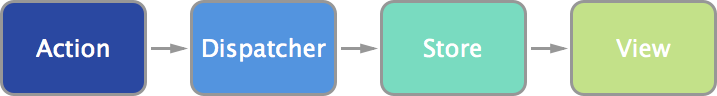
\includegraphics[width=1.0\textwidth]{images/flux.png}
    \caption{Dispatcher, Stores und Views sind unabhängige Knoten mit unterschiedlichen Ein und Ausgaben. Die Aktionen sind einfache Objekte die den Typ und die Daten selbst enthalten.}
    \label{fig:flux}
\end{figure}

Abbildung \ref{fig:flux} zufolge ist es unmöglich, dass eine Component den Zustand der Applikation verändern kann, was jedoch so gut wie immer nötig ist. Hierfür werden die Actions benutzt. Diese können von den Components verwendet werden, um neue Daten an den Dispatcher zu schicken, der sie an den Store weiterleitet. Mittels des Stores kann dann der Zustand verändert werden, siehe Abbildung \ref{fig:flux_actions}.

\begin{figure}[htbp]
    \centering
    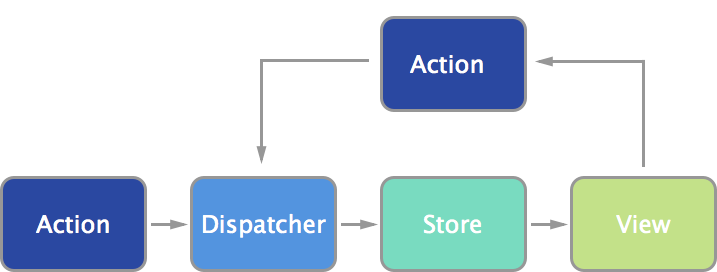
\includegraphics[width=1.0\textwidth]{images/flux_actions.png}
    \caption{Mithilfe von Actions ist die View in der Lage, den Zustand der Applikation, zu verändern.}
    \label{fig:flux_actions}
\end{figure}

Allem in Allem ist die Facebook-Flux Architektur in Kombination mit React.js ein äußerst fortschrittlicher und zukunftssicherer Weg, eine Webapplikation zu schreiben, womit deren Anwendung für die Erstellung des Infoboards als eine gute Wahl erscheint.

\section{Architektur der Applikation}

Wie im vorherigen Abschnitt beschrieben, wurde die Applikation mittels React.js und der Flux-Architektur realisiert. Anstelle der Flux-Implementierung von Facebook, wurde allerdings \textit{reflux} benutzt. Reflux vereinfacht Flux insofern, als dass es keinen einzelnen Dispatcher benutzt. Jede Action ist ihr eigener Dispatcher, mit dem Ziel Flux noch mehr zu vereinfachen und unnötigen Quelltext (sogennanten Boilerplate) zu reduzieren\footnote{Keinen zentralen Dispatcher zu benutzen hat auch Nachteile, für dieses Projekt waren die jedoch nicht von Relevanz.}. Eine Vollständige Erklärung für reflux ist auf dem Blog des Autors zu finden \cite{reflux}. Reflux ist nicht der einzige Versuch, eine Alternative bereitzustellen. Mittlerweile gibt es über 10 verschiedene Flux-Bibliotheken\footnote{Ein Vergleich dieser ist hier zu finden \url{https://github.com/voronianski/flux-comparison}} - mit teilweise großen Gemeinden dahinter oder Firmen wie z.B. \textit{Yahoo} mit \textit{Fluxible}. Der Funktionsinhalt der verschiedenen Flux-Bibliotheken ist mehr oder minder gleich, somit könnte reflux mit Leichtigkeit ausgetauscht werden, wenn es denn nötig wäre.
Die Entwicklung in diesem Bereich ist jedoch äußerst spannend und hat zum Zeitpunkt dieser Arbeit mit redux \cite{gitredux} ihren Höhepunkt gefunden, wo die Stores gar keinen State mehr besitzen und nur noch als Action-Aggregatoren dienen. Dadurch ergibt sich die Möglichkeit, dass der Zustand der Applikation vor- und zurückgespult werden kann, da er rein von den gesendeten Actions abhängig ist\citep{redux}.


\subsection{Überblick}

\begin{figure}[htbp]
    \centering
    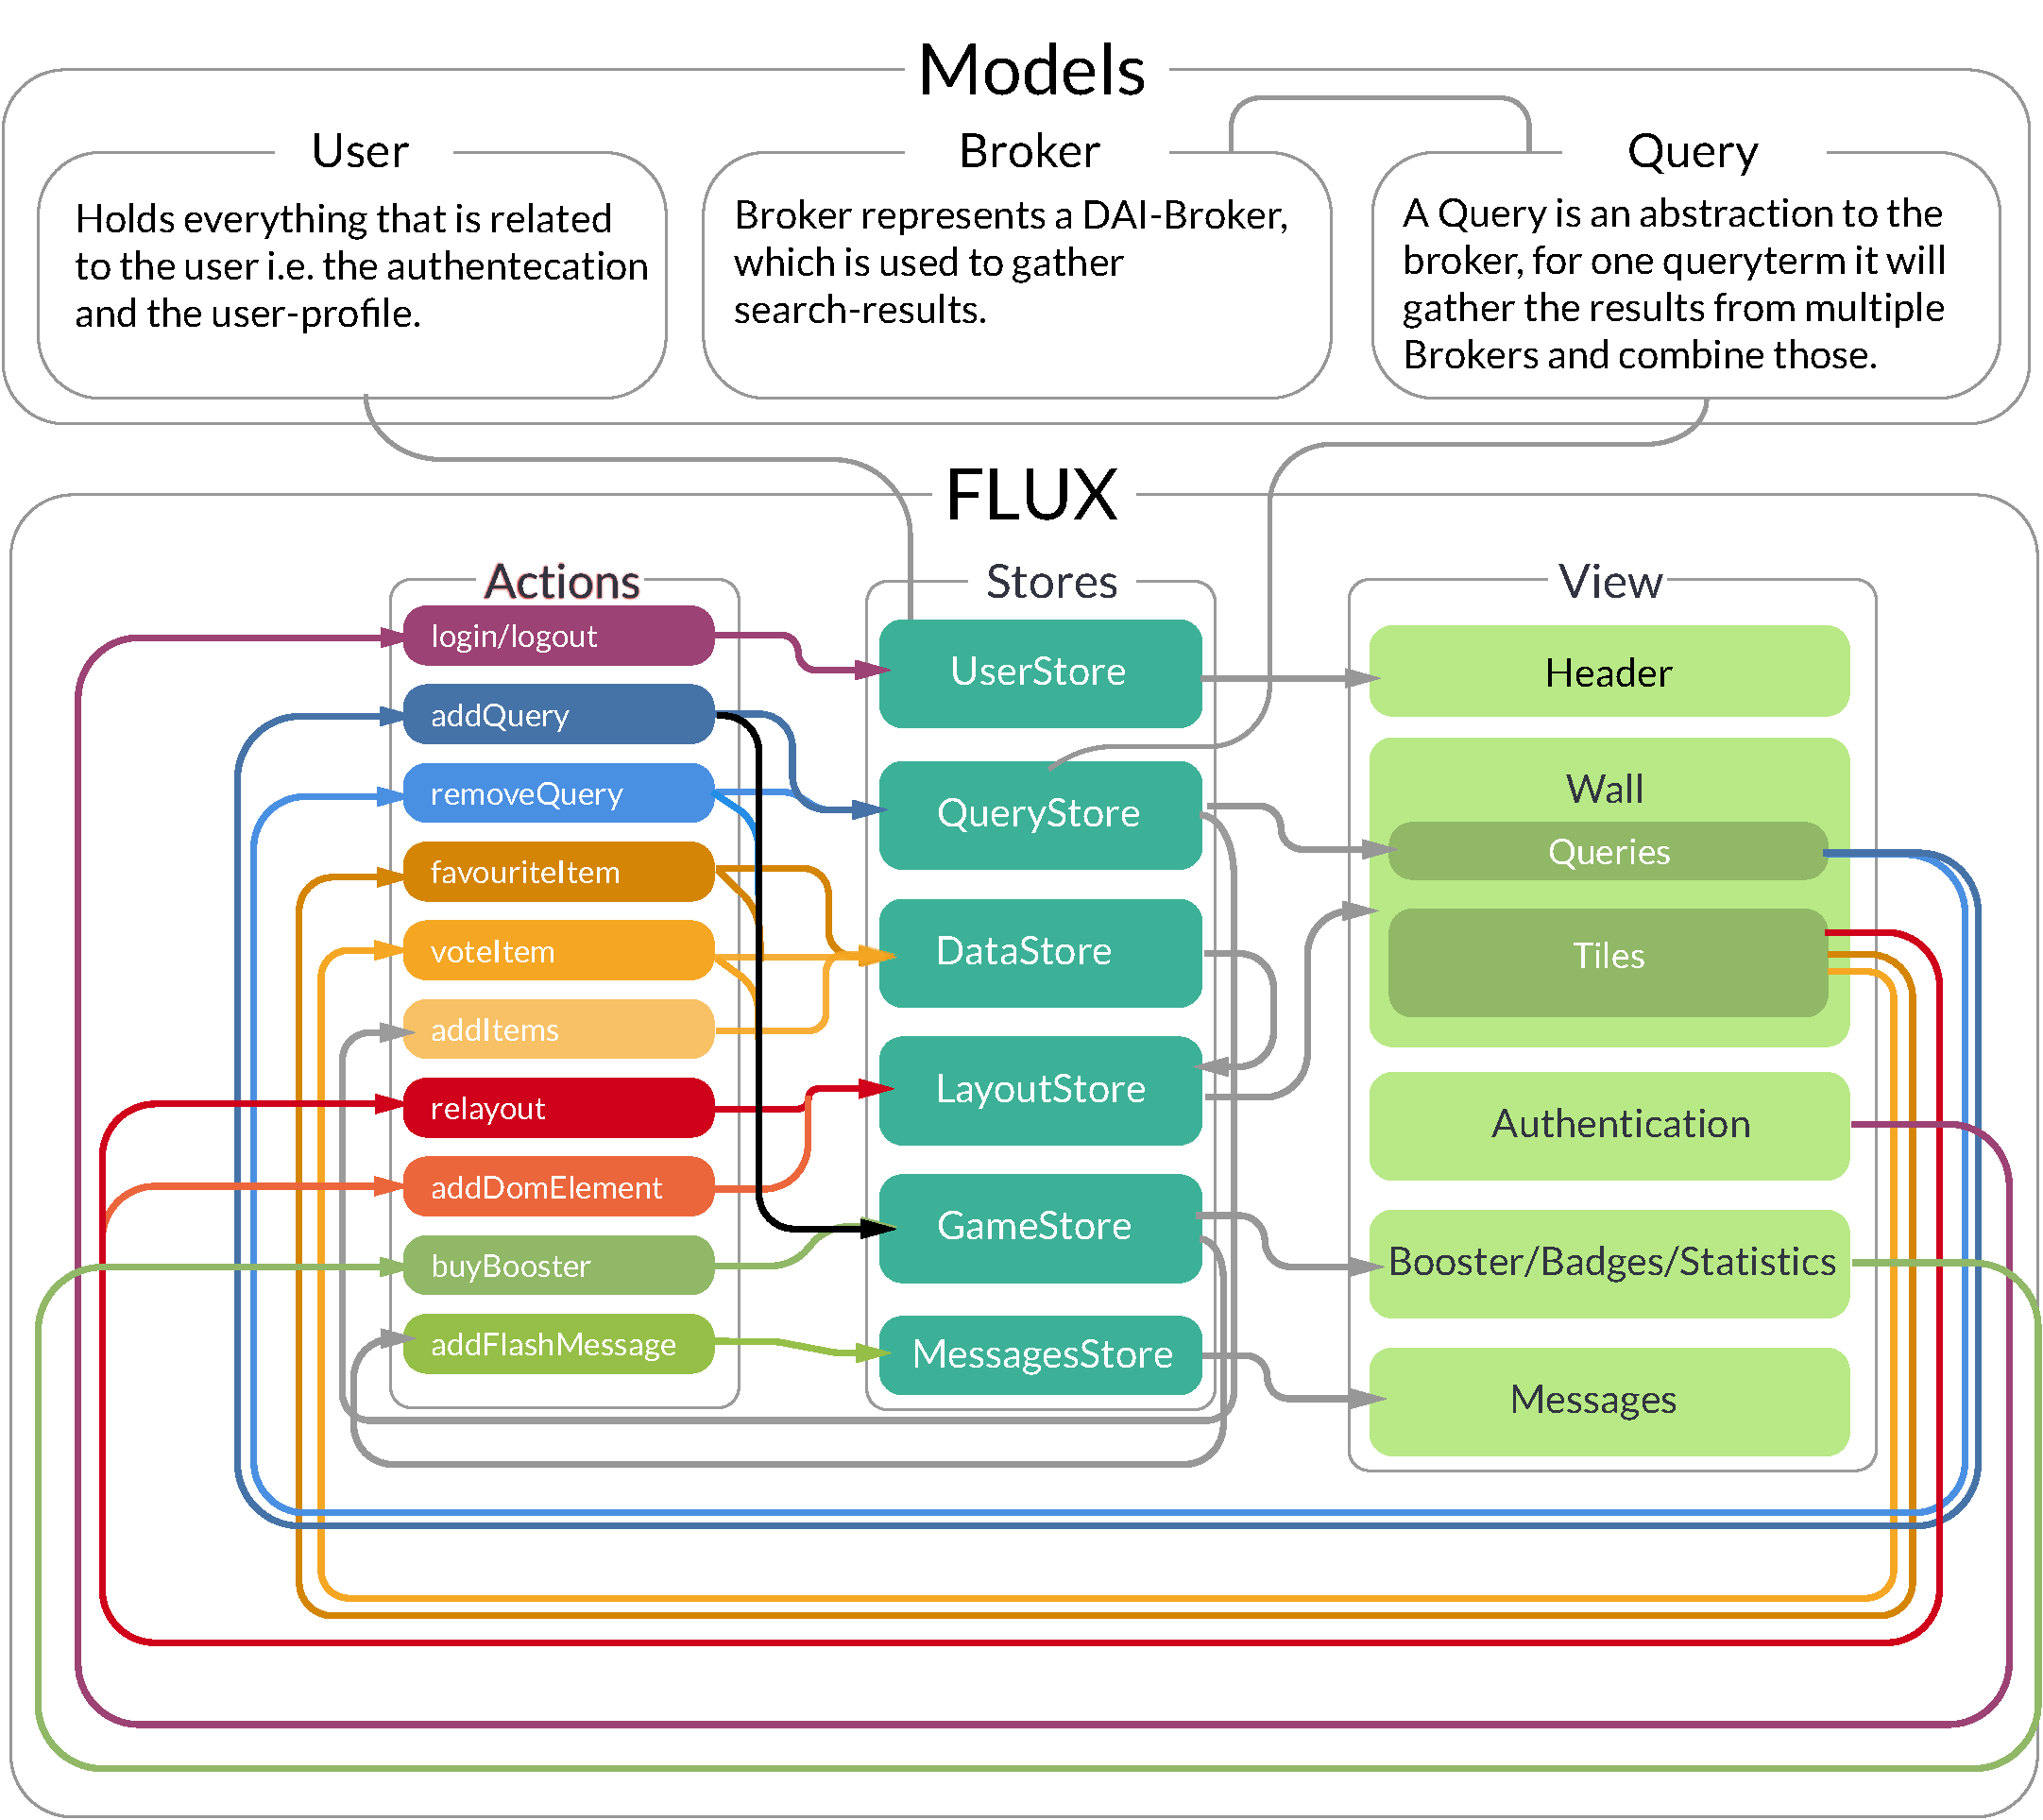
\includegraphics[width=1.0\textwidth]{images/architecture.pdf}
    \caption{Die wichtigsten Bestandteile der Applikation.}
    \label{fig:architecture}
\end{figure}

Die Abbildung \ref{fig:architecture} zeigt einen Überblick über die gesamte Architektur der Infoboard Applikation. Sie wurde bewusst nicht in einem Klassendiagramm dargestellt, da die Applikation keinen strengen objektorientierten Stil verfolgt, und das Schaubild nicht sonderlich zum Verständnis beitragen würde. Dies ist eine grobe Abstraktion, doch reicht die Abbildung, um sich im Quelltext zurecht zu finden.

Es ist deutlich zu sehen, dass der komplette Datenfluss bzw. Programmfluss mittels der Flux-Architektur modelliert wurde, was daran zu erkennen ist, dass jegliche Interaktionen der View mittels Actions an die jeweiligen Stores weitergegeben werden, die dann den neuen Zustand an die View abermals weitergeben.

Zusätzlich zu Flux gibt es noch drei Klassen, die von den jeweiligen Stores benutzt werden, die Auslagerung dieser Logik in eigene Klassen dient der Übersichtlichkeit, verdeutlicht aber auch dass alle Komponenten, mit denen der Benutzer nicht direkt interagiert, nicht Teil des Flux-Datenflusses sein müssen.

\subsection{Stores}

Im folgenden werden die Stores genauer beschrieben.

Die Stores sind zuständig den Datenfluss zu verwalten, insgesamt enthält die Applikation 6 Stores: \texttt{UserStore}, \texttt{QueryStore}, \texttt{DataStore}, \texttt{LayoutStore}, \texttt{GameStore} und \texttt{MessagesStore}.
Der \texttt{UserStore} und \texttt{MessagesStore} sind jedoch äußerst trivial und sind nur wenige Zeilen lang. Die wichtigsten sind die anderen vier, diese werden nun im Detail behandelt.

\subsubsection*{QueryStore}

Der \texttt{QueryStore} abonniert die Aktionen \texttt{addQuery} und \texttt{removeQuery}, er abstrahiert die Anfrage an die \texttt{Broker}, d.h. für jedes Thema werden alle verfügbaren \texttt{Broker} angefragt. Nach jeder Antwort eines solchen wird die Nachricht \texttt{addItems} mit den Ergebnissen gesendet. Auf diese Nachricht hört der \texttt{DataStore}.

\subsubsection*{GameStore}

Der \texttt{GameStore} liefert alles, was für die Verspielisierung der Applikation relevant ist - wie die Bereitstellung der Punkte, der Bestenlisten und Trophäen aller Benutzer der Applikation. Weiterhin abonniert er alle Aktionen auf denen Punkte definiert sind, wie das Bewerten eines Suchergebnisses und sorgt dafür, dass diese Aktionen vom Backend verarbeitet werden.

Um den sozialen Faktor zu erhöhen, reagiert der \texttt{GameStore} ebenfalls auf die Aktionen aller anderen Benutzer. Dies geschieht quasi in Echtzeit und sorgt dadurch z.B. für eine äußert lebendige Statistikseite (auf dieser werden die Daten aller Benutzer angezeigt).
Damit das ganze noch effizient bleibt, wurden WebSockets verwendet, die deutlich weniger ``Overhead'' besitzen als normale HTTP-requests.

\subsubsection*{DataStore}

Der \texttt{DataStore} stellt alle Daten bereit, die für die Darstellung benötigt werden. Das sind in der Regel die Suchergebnisse, die mit dem Profil des Benutzers verbunden werden, um anzuzeigen, welche Ergebnisse bewertet/favorisiert wurden, und die Suchanfragen, die zur Laufzeit verändert werden können. Herausforderungen hier waren es, Duplikate in den Suchergebnissen zu verarbeiten sowie die Interaktion mit den Suchergebnissen.

Hierzu hört er auf die Nachricht \texttt{addItems}, welche eine Liste mit Suchergebnissen enthält. Diese Daten sind noch ganz ohne die Bewertungsdaten, welche hier angefragt werden und in die Suchergebnisse integriert werden. Sobald das geschehen ist, wird allen Abonnenten (in dem Fall der \texttt{LayoutStore} mitgeteilt, dass der Datensatz sich verändert hat.

Eine Besonderheit ist die Benutzung einer nicht veränderbaren \texttt{OrderedMap}, in der die Suchergebnisse mit ihrer URL als Schlüssel gespeichert sind. Die Suchergebnisse werden in der Applikation noch viel weitergereicht, weswegen viele Fehler vorgebeugt werden, da nur der \texttt{DataStore} selbst die Suchergebnisse verändern kann.

\subsubsection*{LayoutStore}

Im Design-Abschnitt wurde ausführlich darauf eingegangen, was die Layouting-Engine alles leisten muss, leider konnte keine der OpenSource-Bibliotheken allen Anforderungen gerecht werden. Deswegen wurde für die Darstellung eine eigene Layouting-Engine erstellt.
Die Grundlage ist die absolute Positionierung innerhalb des Browsers, diese ist notwendig um Animationen zu ermöglichen. Es gibt verschiedene Arten, DOM-Elemente durch CSS zu positionieren:

\begin{enumerate}
  \item Mithilfe von \texttt{top/left}.\\
  \begin{minted}{css}
  .position-top-left {
      position: absolute; /* or relative/fixed */
      top:  50px;
      left: 50px;
  }
  \end{minted}
  \item Mithilfe von \texttt{transform: translate(x, y)}. Dies ist allgemein anerkannt schneller zu sein und hat den Vorteil, dass subpixel-animationen möglich sind, was im Allgemeinen flüssigere Animationen erlaubt \cite{translate}. \\
  \begin{minted}{css}
  .position-translate {
      position: absolute; /* or relative/fixed */
      transform:         translate(50px, 50px);
      -webkit-transform: translate(50px, 50px);
  }
  \end{minted}
  \item Mithilfe von \texttt{transform: translate3D(x, y, z)}. Dies ist mit Abstand der schnellste Ansatz \cite{translate3dvstranslate}. Hierbei werden die Elemente zu Texturen gerendert und mit Einsatz des Grafikprozessors animiert. Dadurch ist es sogar möglich, auf mobilen Endgeräten flüssige Animationen zu gewährleisten, da diese gewöhnlich dedizierte Grafikprozessoren besitzen.
  \begin{minted}{css}
  .position-translate3D {
      position: absolute; /* or relative/fixed */
      transform:         translate3D(50px, 50px, 0);
      -webkit-transform: translate3D(50px, 50px, 0);
  }
  \end{minted}
  \texttt{transform3D} wird von allen aktuellen Browsern soweit unterstützt, dass unser Szenario möglich ist\cite{transform3d}. Was weiterhin zu beachten ist, dass am Ende immer gerundete Pixelwerte innerhalb von \texttt{translate3D(x, y, z)} benutzt werden sollten, weil die Elemente ansonsten unscharf sind, siehe Abbildung \ref{fig:blurry}.

\begin{figure}[htbp]
	\centering
	
\includegraphics[width=1.0\textwidth]{images/blurry_tiles.png}
	\caption{Links eine Kachel mit geraden Werten bei \texttt{translate3D}, rechts mit jeweils $.5$ bei $x/y$.}
	\label{fig:blurry}
\end{figure}

\end{enumerate}

Es ist eine Grundanforderung Geräte mit unterschiedlich großen Bildschirmen zu unterstützen, was dadurch erzielt wird, dass die Anzahl der Spalten variabel ist.
Es gibt zwei Möglichkeiten, die Anzahl der Spalten variabel zu machen:

\begin{enumerate}
  \item Berechne die Breite mittels Javascript bevor das Element in den DOM eingefügt wird und setze die Breite mittels style-Attribut.
  \item Durch die Benutzung von \textit{Media Queries} können direkt in CSS verschiedene Darstellungen für unterschiedliche Bildschirmbreiten beschrieben werden.
\end{enumerate}

Für die Positionierung müssen, wir wissen wie viele Spalten zu jedem Zeitpunkt dargestellt werden sollen. Dafür muss die Breite in Javascript berechnet werden, somit liegt 1. nahe. Von uns durchgeführte Versuche haben jedoch gezeigt, dass es schneller ist, die Breite des Elementes nicht per Javascript zu setzen, sondern diese über die \texttt{Media Queries} zu bestimmen. Zwar bedeutet dies, dass die gleiche Logik an zwei Orten in 2 Sprachen steht, aber da das nicht mehr als jeweils 10 Zeilen sind, ist es für die resultierende bessere Geschwindigkeit hinnehmbar.

Die Breite aller Elemente ist zu jedem Zeitpunkt gleich, die Höhe ist jedoch variabel. Da es unmöglich ist, die Höhe auszurechnen, ohne eine komplette Browser-Engine zu implementieren, muss das Element in den DOM eingefügt werden, bevor wir dessen korrekte y-Position berechnen können. Hierfür existiert die Aktion \texttt{addDOMElement}, welche die gleichnamige Funktion im \texttt{LayoutStore} ausführt. Diese Funktion ist neben der \texttt{relayout}-Funktion der einzige Ort, an dem der DOM direkt ausgelesen wird, nämlich die Höhe des Elementes mit \texttt{offsetHeight}. Solange kein \texttt{resize}-Event getriggert wird, muss dieser Wert auch nicht ein zweites Mal ausgelesen werden.
Wenn es zu allen Suchergebnissen eine Kachel gibt, wird die \texttt{layout}-Funktion aufgerufen, womit die korrekte Position der Kacheln ausgerechnet wird und auf diese weitergegeben wird.

Der vollständige Programmfluss ist komplex, da er sehr auf Geschwindigkeit getrimmt wurde. Der Programmteil ist ausführlich kommentiert und beschrieben.

Allgemein hat die Flux-Architektur hier gut funktioniert. Das größte Manko entstand beim Abgleichen des LayoutStores mit dem \texttt{DataStore}. Wenn nun ein Element positiv bewertet wird, muss das Layout neu berechnet werden. Der LayoutStore weiß nicht direkt, welches Element sich verändert hat, es muss durch alle Elemente des \texttt{DataStores} mit den Eigenen abgleichen. Dies ist nicht unbedingt optimal, allerdings stellt sich die Frage, ob eine andere Architektur das Problem einfacher lösen würde.

\subsection{Views}

Als View wird das Interface bezeichnet, mit dem der Benutzer schlussendlich interagiert. Für jedes View wird React.js und React-Bootstrap verwendet. Die Gründe, warum React.js verwendet wird, sind in Abschnitt \ref{sec:flux} genauer ausgeführt.

\subsubsection*{Responsives Design}

Responsives Webdesign bezeichnet ein Paradigma, bei dem Webseiten daraufhin geschrieben werden, dass die Darstellung der Inhalte auf unterschiedlichen Geräten, ohne Einbußen in der Benutzerfreundlichkeit möglich ist. Praktikabel bedeutet das, dass die Darstellung abhängig von der Bildschirmbreite des Gerätes ist. \cite{natda2013responsive}.

Aktuell wird das so umgesetzt, dass jeglicher Inhalt mit der Benutzung eines \textit{Grid}-Systems dargestellt wird. Grid-Systeme werden benutzt, um ``... Seitenlayouts mittels Zeilen und Spalten, die Inhalte aufnehmen, zu kreieren.'' (\cite{bootstrap}, übersetzt aus dem Englischen).

Eine genaue Erklärung von Grid-Systemen ist nicht im Rahmen der Arbeit, für mehr Informationen zu Grid-Systemen wird auf \cite{bootstrap} verwiesen.
In dieser Applikation wird das von Bootstrap bereitgestellte Grid intensiv benutzt, um auf jedem Endgerät eine möglichst gute Benutzererfahrung zu garantieren.

\subsubsection*{Erstellte React.js-Komponenten}

Wie auch in anderen Interface-Bibliotheken wird in React.js das Interface in Komponenten unterteilt (in anderen Bibliotheken auch \textit{widgets} gennant).

An dieser Stelle wurde überlegt, eine Einführung in React.js zu schreiben, jedoch würde auch dies die Ansprüche dieser Arbeit übersteigen. Stattdessen wird auf das offizielle Tutorial von Facebook verwiesen \cite{tutorial}.

Es wurden 30 React-Komponenten erstellt, viele davon sind nicht anwendungsspezifisch und wurden an mehreren Stellen der Applikation verwendet. Unterteilt sind sie semantisch nach Aufgabe/Seiten, wie zum Beispiel \texttt{settings}, \texttt{stats} oder \texttt{utility}.
Eine Minimalübersicht findet sich in Abbildung \ref{fig:architecture}, in welchem alle Komponenten gezeigt werden die Teil des Flux-Kreises sind, alle Restlichen sind statisch und spielen für die Architektur keine Rolle.

Die erstellten Seiten sind in den Abbildungen \ref{fig:booster}, \ref{fig:settings}, \ref{fig:stats} und \ref{fig:badges} zu sehen.

Die wichtigste Seite ist die mit der eigentlichen Applikation, nämlich das Infoboard bzw. das Interface für das Suchen von Informationen mittels Themen, zu sehen in Abbildung \ref{fig:wall}. Der Benutzer wird sich voraussichtlich die meiste Zeit auf dieser Seite befinden, deshalb sind auch alle relevanten Aktionen, neben dem Einloggen und dem Kaufen von Boostern, nur auf dieser Seite möglich. Für weitere Details zu dem Konzept dieser Seite, siehe Abschnitt \ref{chap:concept:wall}.

Neben der Seite mit dem Infoboard, sind noch 4 weitere Seiten verfügbar. Diese dienen hauptsächlich der Gamification. Für den Nutzer am interessantesten ist die Seite mit den Benutzerstatistiken, zu sehen in Abbildung \ref{fig:usersite}.
Weiterhin gibt es noch die Seite, auf dem der Benutzer den derzeitigen Status seines aktuellen Boosters sehen kann, und falls er keinen hat, die Möglichkeit besitzt, einen neuen Booster zu erwerben, siehe Abbildung \ref{fig:booster}. Einstellungen, wie das Auswählen des Farbschemas, kann der Nutzer ebenfalls auf einer dedizierten Seite tätigen, siehe Abbildung \ref{fig:settings}.

Eine allgemeine Übersicht der Aktivität aller Nutzer ist auf der Statistik-Seite zu sehen. Diese Seite ist dafür gedacht, auf einem Fernseher, der in einem öffentlichen Raum des Betriebes aufgehängt ist, angezeigt zu werden. Die Seite unterteilt sich in drei Abschnitte. Der erste Teil zeigt zwei Bestenlisten an, eine für den kompletten Zeitraum und eine für den letzten Monat. Im zweiten Teil ist die Gesamtpunktzahl der Mitarbeiter zu sehen. Wie auf der Seite mit den Benutzerstatistiken, ist sie aufgeteilt in die einzelnen Kategorien. Der Dritte Teil besteht aus einem Livestream der Nutzeraktivitäten, jedes Mal wenn eine Aktion ausgeführt wurde, dort anzeigt. Die Seite ist zu sehen in Abbildung \ref{fig:stats}.

Der Aufbau der eigentlichen Komponenten, wird Beispielhaft in Appendix \ref{chap:appendix:component} anhand der \texttt{Query}-Komponente gezeigt.

\section{Backend}\label{sec:backend}

Im Verlaufe der Arbeit wurde erkannt, dass eine dedizierte Backend-Applikation nötig ist, um den Grad der Interaktion und der Dynamik zu ermöglichen, die als Ziele gesetzt wurden. Es gibt einige Frameworks, die zur Frage standen, aber schließlich fiel die Entscheidung auf node.js, da dadurch die Möglichkeit bestand, einiges an Quelltext mit dem Frontend zu teilen. Das node.js \textit{non-blocking} ist und \textit{event-driven IO} benutzt, macht es vorteilhaft für Applikationen, die viele Anfragen verarbeiten müssen \citep{tilkov2010node}. Anders als in klassischen Frameworks wie rails oder django, wo bei jeder Anfrage ein neuer Thread aufgemacht wird, der solange blockiert ist, bis er abgehandelt wurde, wird jede Anfrage von einem \textit{event-loop} beantwortet \citep{tilkov2010node}. Alles in node.js ist asynchron, weswegen diese Anfragen nicht blockieren. Damit ist es mit node.js möglich, bis zu 1 Million Verbindungen zeitgleich zu halten \cite{node1m}.

Als Datenbank wurde mysql verwendet, die durch einem Object Relationship Mapper (kurz ORM) angesteuert wird. Mit einem ORM ist es möglich, Datenbanken mittels Klassen und Objekten zu abstrahieren. Ein ORM ist jedoch nur eine einfach Abstraktion und beherrscht nicht alle Funktionalitaten SQLs, jedoch reichen die Fähigkeiten des ORMs meistens aus und es kann immer auf direkte SQL-Anfragen zurückgegriffen werden. Das hier Verwendete ORM ist sequelize \cite{sequelize}. Als Datenbank wird mysql verwendet, da viel internes Knowhow mit dieser Datenbank bestand. Es können aber ohne Einschränkungen andere von sequelize unterstützte Datenbanken benutzt werden.

Das verwendete Datenmodell kann in Abbildung \ref{fig:database} betrachtet werden, es ist komplett mit sequelize beschrieben und ist damit ohne viel Aufwand veränderbar.

\subsection{HTTP-API}

Die Kommunikation von Backend und Frontend geschieht per HTTP-Anfragen, das verwendete Framework ist express.js, es wurde überlegt ein API-Framework wie Swagger \cite{swagger} zu benutzen. Diese erstellen eine einheitliche, sich selbst-aktualisierende Dokumentation wie auch einfache Tests \cite{haupt2014model}.
Damit wäre jedoch eine weitere Technologie eingeführt worden und da sich die Anzahl der Endpunkte nur auf 8 beläuft, haben wir uns bewusst dagegen entschieden. Im folgenden wird Schemenhaft der Ablauf der Anfragen aller Endpunkte illustriert.

\begin{description}
	\item[\texttt{POST  /user/action}] Jede Aktion des Benutzers wird an diesen Endpunkt gesendet der folgenden Ablauf besitzt:
	\begin{enumerate}
		\item Finde den angegebenen Benutzer in der Datenbank
		\item Suche alle Booster des Benutzers und finde heraus ob einer aktiv ist
		\item Füge die Aktion in die Datenbank ein, wenn ein Booster aktiv ist, multipliziere die Punkte der Aktion mit dessen Multiplikator
		\item Falls die Aktion auf einem Suchergebnis statt fand, verknüpfe dieses mit der Aktion
		\item Berechne die Abzeichen neu, wenn sich diese von den bisherigen Abzeichen unterscheiden, füge die neuen in die Datenbank ein und füge sie der Antwort hinzu
		\item Antworte mit der erstellten Aktion und ggf. mit den erstellten Abzeichen
	\end{enumerate}
	\item[\texttt{POST /user/vote}] Sobald der Benutzer ein Suchergebnis bewertet, wird diese Anfrage gesendet. Der folgende Ablauf findet statt:
	\begin{enumerate}
		\item Finde den angegebenen Benutzer in der Datenbank
		\item Finde das angegebene Suchergebnis in der Datenbank und erstelle es neu falls nicht vorhanden.
		\item Finde die bisherige Bewertung des Suchergebnissen oder erstelle diese neu falls nicht vorhanden.
		\item Setze den neuen Wert für die Bewertung und speichere diese
		\item Antworte mit der erstellten Antwort
	\end{enumerate}
	\item[\texttt{POST /user/booster}] Sobald der Benutzer einen Booster erwirbt wird mittels dieser Anfrage die Transaktion in der Datenbank festgehalten. Dazu wird der angegebene Benutzer gesucht und der gekaufte Booster erstellt.
	\item[\texttt{GET /points}] Diese Anfrage nimmt zwei Parameter, Anfangsdatum und Enddatum. Das Ergebnis ist eine Liste aller Benutzer mit ihren jeweiligen Punkten und Abzeichen, zusätzlich werden die Punkte aller Nutzer Kategorieunterteilt und komplett aufsummiert zurückgeliefert.
	\item[\texttt{GET /items}] Diese Anfrage nimmt als Parameter eine Liste an Suchergebnissen-URLs und findet alle Bewertungen und Aktionen auf das Suchergebnis zeigen. Die Bewertungen werden aufsummiert.
	\item[\texttt{GET /actions}] Diese Anfrage liefert die letzten 50 Aktionen zurück.

\end{description}

\subsection{Websockt-API}

Um die Dynamik des Infoboards zu maximieren wurden Websockets verwendet die auf alle ausgeführten Aktionen des Systems reagieren und dadurch z.B. die Gesamtpunktzahl erhöhen. Websockets wurden jedoch nicht in ihrer reinen Form benutzt, sondern mittels der Bibliothek socket.io \cite{rauch2013socket}. Diese ermöglicht neben einer einfacheren Benutzung von Websockets, auch einen Alternativmodus mittels polling um Geräte zu unterstützen, die keine Websockets besitzen.


\chapter{Fazit und Ausblick}

Viele Technologien, die in dieser Arbeit genutzt wurden, sind vor wenigen Jahren noch nicht denkbar gewesen. Da der Maturitätsgrad dieser nicht sehr hoch ist, ist die Nutzung dieser auch mit Risiken verbunden. Das Entwickeln der Applikation war damit zu einem gewissen Teil eine Fallstudie für neue Technologien in der Webentwicklung.
Rein technologisch betrachten ist die Arbeit jedoch ein voller Erfolg. Sie ist performant, ästhetisch anspruchsvoll und die unidirektionale Architektur übersichtlich und erweiterbar.
Wenn man nach den am Anfang der Arbeit gesetzten Anforderungen geht, erfüllt das Ergebnis diese vollständig.

Doch sind Softwaresysteme schwer nach dem Papier zu beurteilen, gerade wenn es sich um Interface-getriebene Systeme handelt. Das Interface wurde nach aktuellsten Praktiken im Bereich der Benutzererfahrung erstellt und besonders die Darstellung der Suchergebnisse entstand in einem langen iterativen Prozess und stellt etwas dar das so vorher noch nicht existiert hat, aber ob diese nun auch eine wirkliche Innovation darstellt muss erst noch herausgefunden werden. Mehr Funktionalität in einem Produkt bedeutet nicht dass es besser ist als das Vorherige.

Die Implementierung der Gamification wurde nach aktueller Theorie betrieben und programmiertechnisch besitzt sie keine offensichtlichen Mängel, jedoch muss eine wissenschaftliche Analyse betrieben werden um zu zeigen ob diese nun die gewünschten Effekte erzeugt.

Wie jedes Softwaresystem ist auch dieses nie im finalen Entwicklungsstadium, sondern wird ständig weiterentwickelt. Es gibt viele Aspekte wie zum Beispiel die Darstellung der Statistiken, Optimierung der Gamification, Implementierung von Zugriffsrestriktionen oder  die Bereitstellung von neuen Darstellungsformen für die Suchergebnisse die noch behandelt werden können. Allgemein ist das Thema Gamification im Unternehmensbereich um Wissensaustausch zu Fördern ein interessantes Gebiet, dass noch viel Potential birgt.

% Abschließend sei gesagt, dass die Autoren hoffen, dass diese Arbeit, was das Testen von neuen Technologien angeht nicht unbeachtet bleibt, und das dieser Arbeit zugrundeliegende Projekt als Beispiel für zukünftige Projekt genommen wird.
\newpage

\pagenumbering{roman}
\setcounter{page}{\thesavepage}
\addcontentsline{toc}{chapter}{Literaturverzeichnis}
\printbibliography
\cleardoublepage

\addcontentsline{toc}{chapter}{Abbildungsverzeichnis}
\listoffigures
\cleardoublepage
\addcontentsline{toc}{chapter}{Abkürzungsverzeichnis}
\chapter*{Abkürzungsverzeichnis}

\begin{tabbing}
    RSS \hspace{3cm} \= Rich  Site Summary \kill
    PDF \> Portable Document Format \\
    RGB \> Rot Grün Blau  (Farbraum) \\
    HSL/HLS \> Hue, Saturation, Luminance \\
    HSV \> Hue, Saturation, Value \\
    Lab/CIELAB \> Farbraum der Internationalen Beleuchtungskommission \\
    HCL/CIELUV \> Farbraum der Internationalen Beleuchtungskommission \\
    HUSL \> human-friendly HSL \\
    GWT \> Google Web Toolkit \\
    ECMA \> European Computer Manufacturers Association \\
    ES \> ECMAScript \\
    CSS \> Cascading Style Sheets \\
    DOM \> Document Object Model \\
    MVC \> Model View Control \\
    ORM \> Object Relationship Mapper \\
    HTTP \> Hypertext Transfer Protocol
\end{tabbing}
\cleardoublepage

\addcontentsline{toc}{chapter}{Anlagen – Inhalte der beiliegenden CD}
\chapter*{Anlagen – Inhalte der beiliegenden CD}
\begin{itemize}
	\item Quelltext
\end{itemize}

\addcontentsline{toc}{chapter}{Appendix}
\chapter*{Appendix}

\addcontentsline{toc}{section}{Abbildungen}
\section*{Abbildungen}


\begin{figure}[htbp]
    \centering
    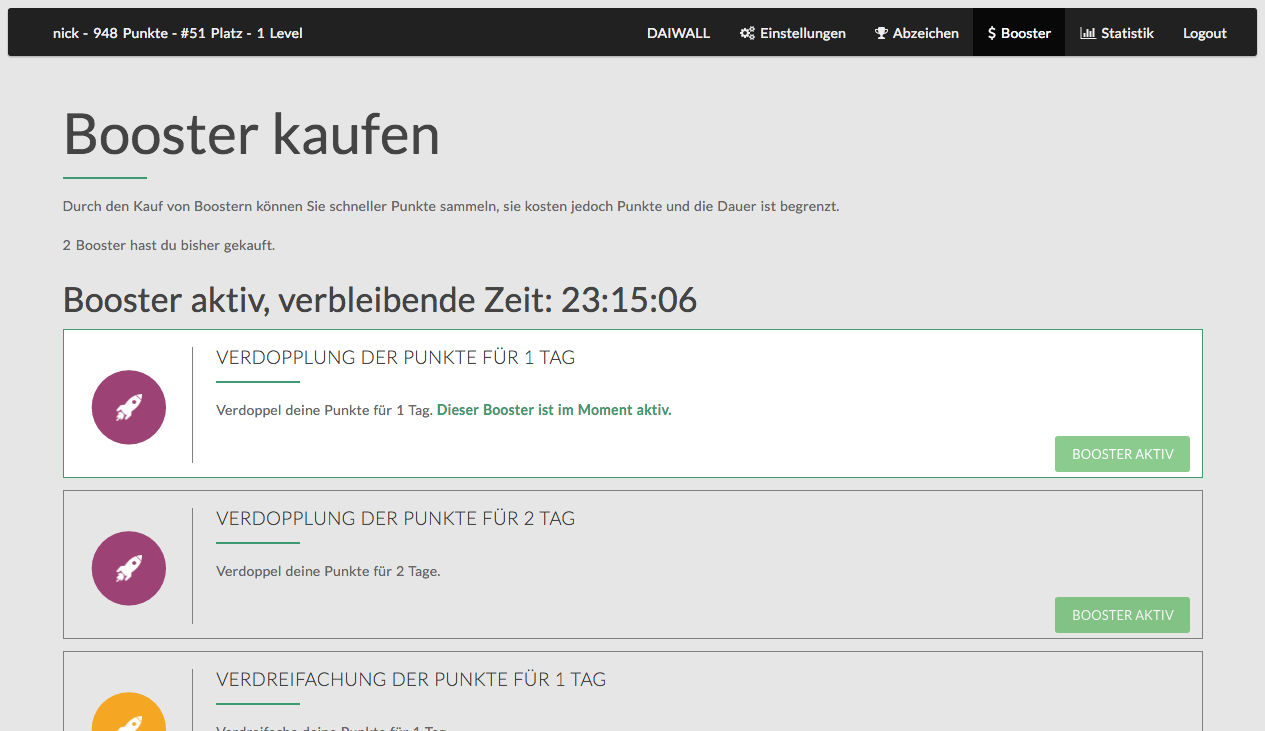
\includegraphics[width=1.0\textwidth]{images/infoboard_booster.png}
    \caption{Auf dieser Seite kann der Benutzer verschiedene Booster erwerben und sehen, wie lange der Aktuelle noch aktiv ist.}
    \label{fig:booster}
\end{figure}

\begin{figure}[htbp]
    \centering
    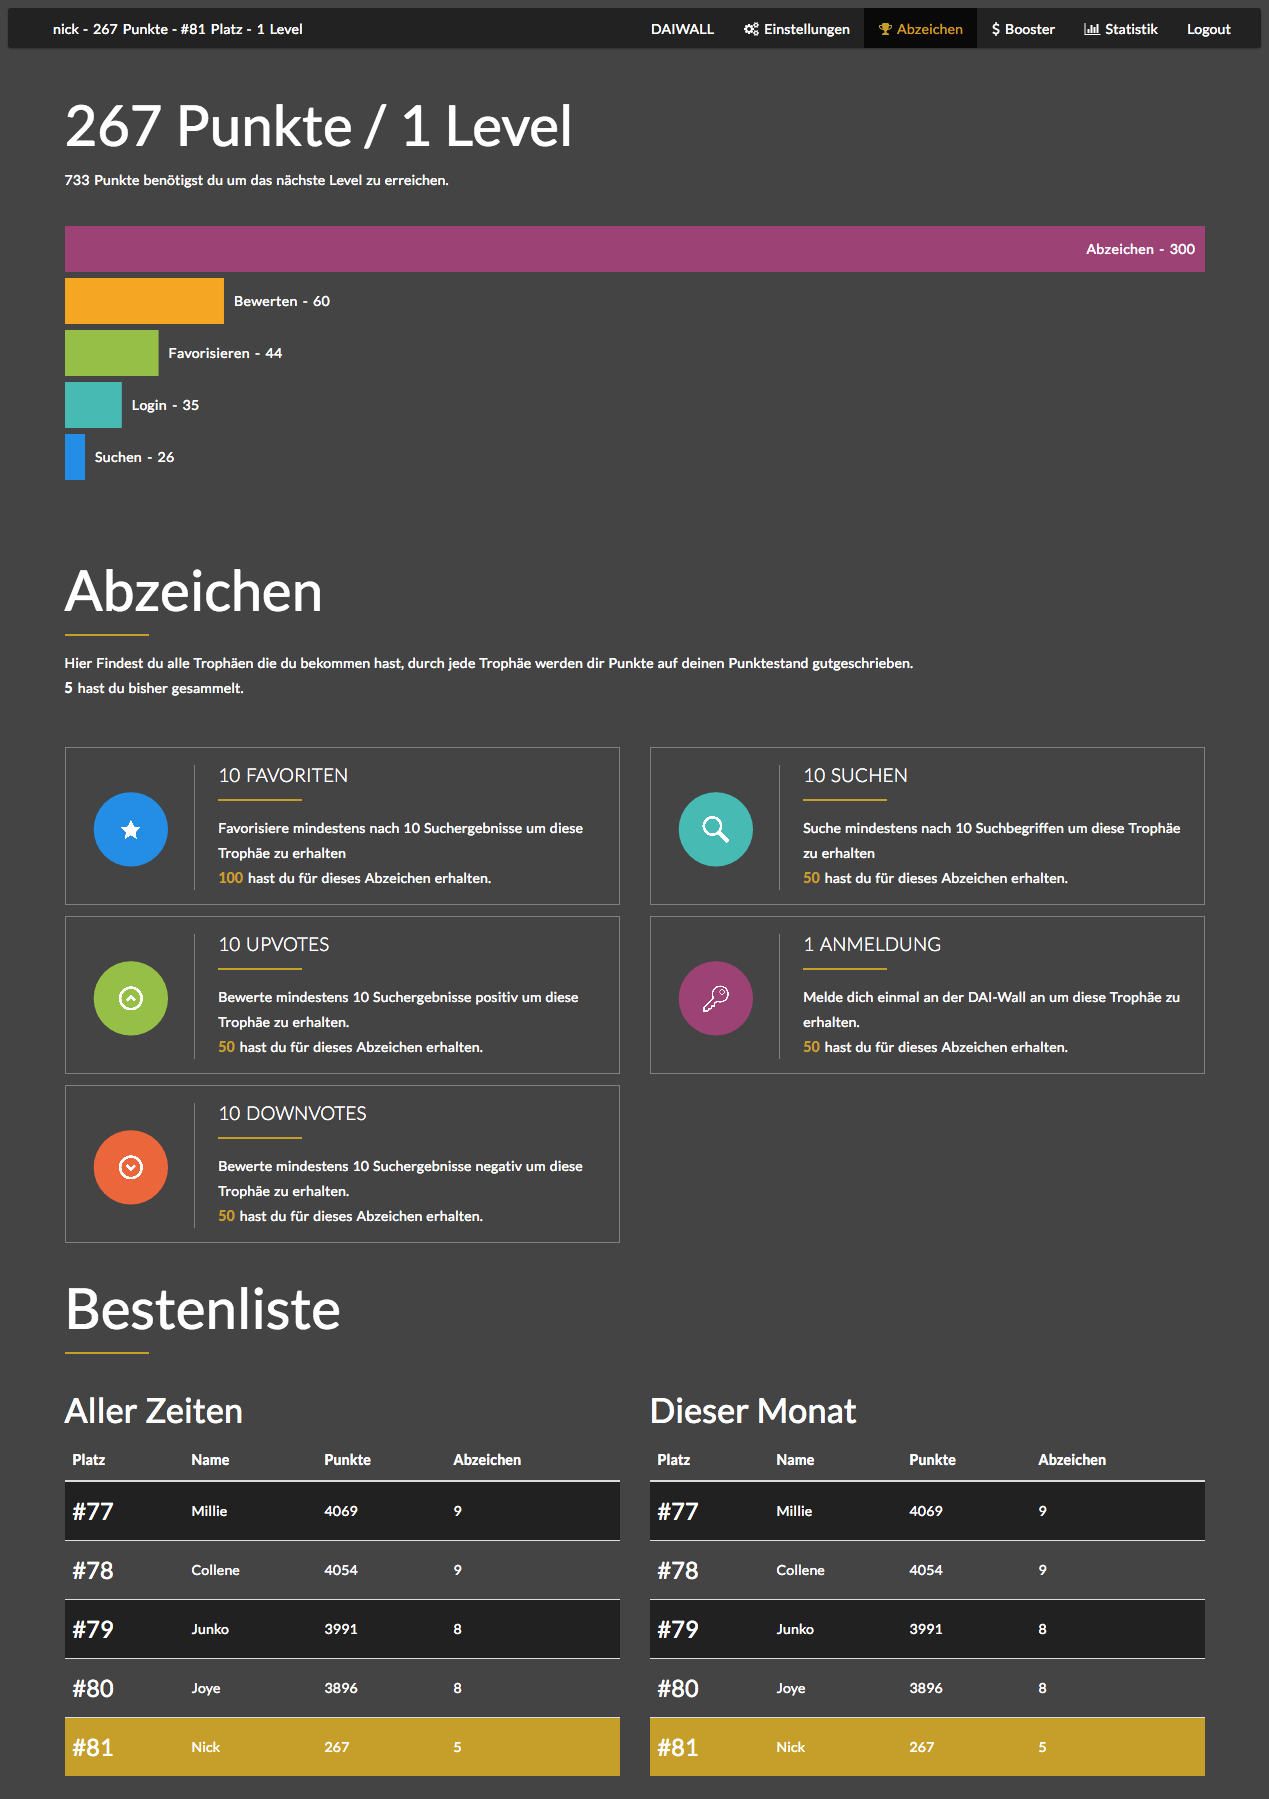
\includegraphics[width=1.0\textwidth]{images/infoboard_usersite.png}
    \caption{Auf dieser Seite kann der Benutzer einsehen, wie viele Punkte er hat, wie sie aufgeteilt sind, welche Abzeichen er besitzt und welche Personen direkt über oder unter ihm auf der Bestenliste stehen. }
    \label{fig:usersite}
\end{figure}

\begin{figure}[htbp]
    \centering
    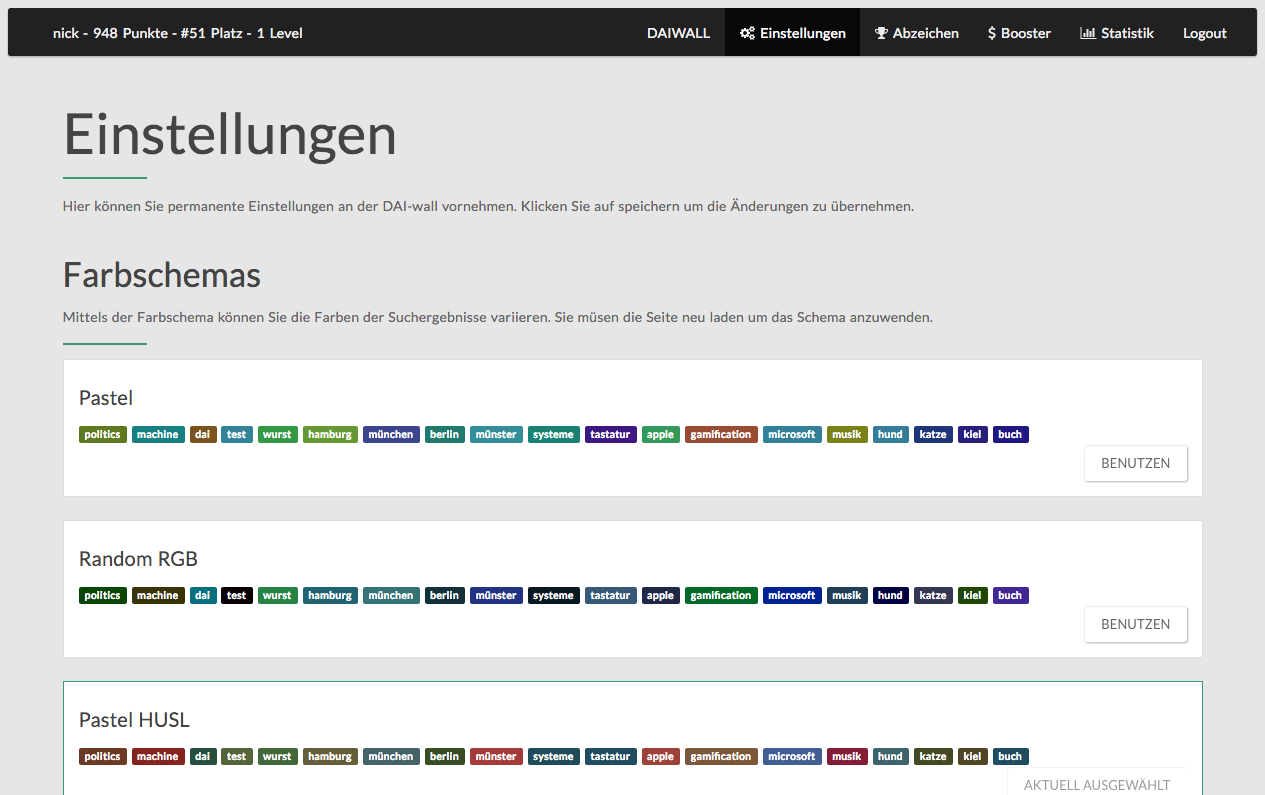
\includegraphics[width=1.0\textwidth]{images/infoboard_settings.png}
    \caption{Auf dieser Seite kann der Benutzer sämtliche Parameter für das Infoboard einstellen. Im Moment beschränkt sich dies auf die Auswahl des Farbschemas, welche jeweils erst nach dem erreichen eines bestimmten Levels verfügbar sind.}
    \label{fig:settings}
\end{figure}


\begin{figure}[htbp]
    \centering
    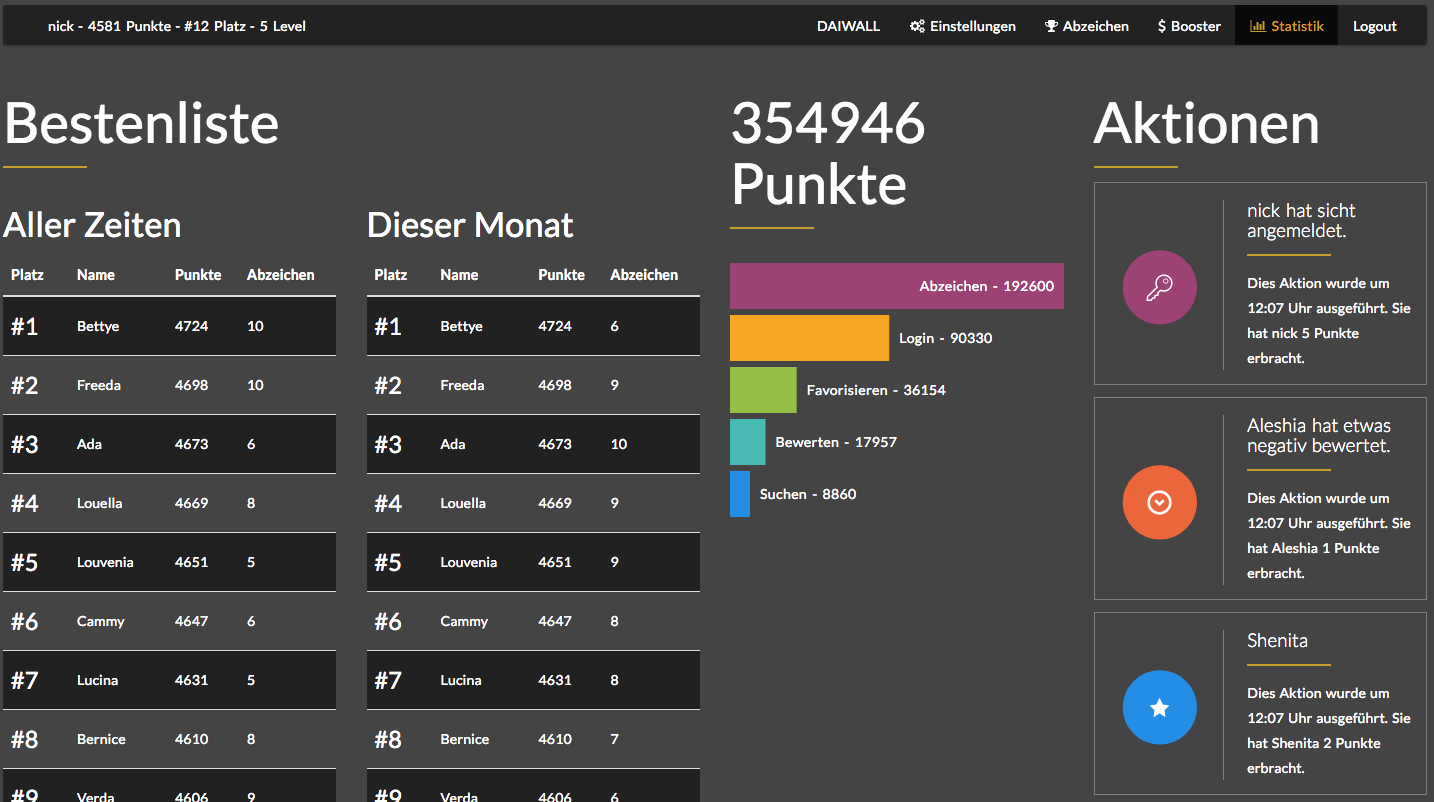
\includegraphics[width=1.0\textwidth]{images/infoboard_stats.png}
    \caption{Die Gesamtstatistikseite. Um den Effekt der Gamification zu erhöhen, sollte diese an einem öffentlichen Ort des Betriebs permanent gezeigt werden.}
    \label{fig:stats}
\end{figure}

\begin{figure}[htbp]
    \centering
    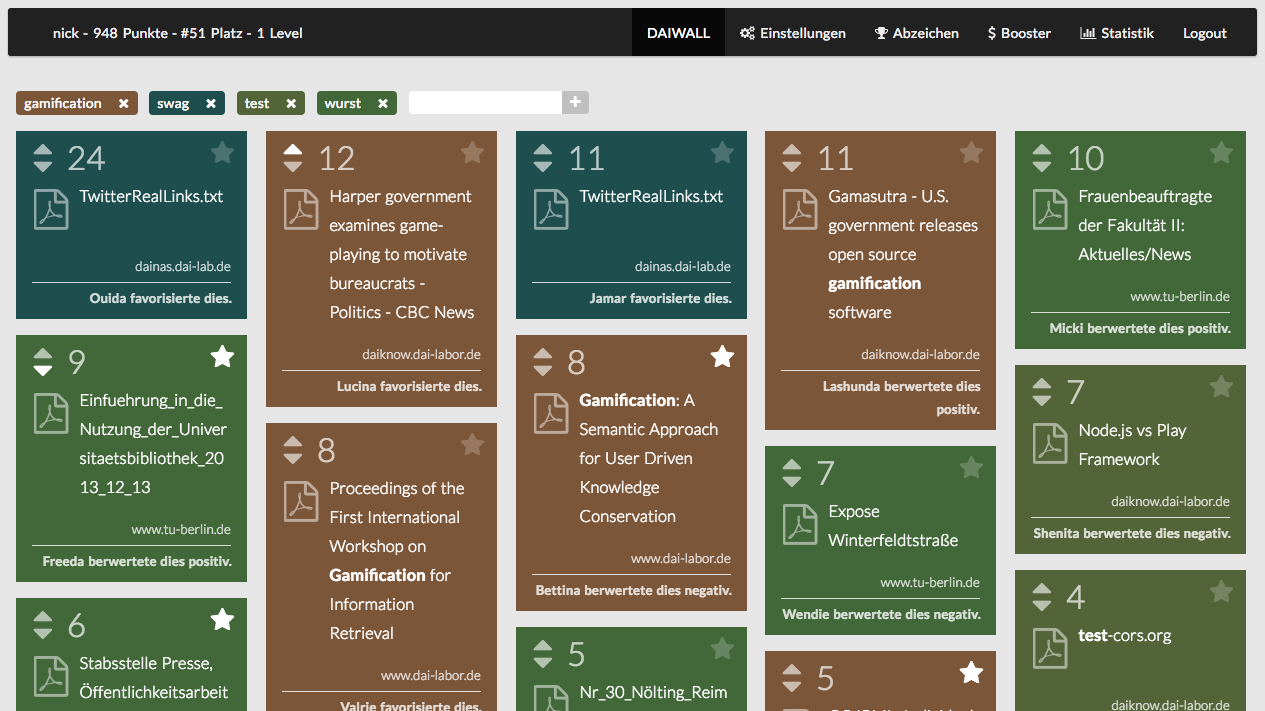
\includegraphics[width=1.0\textwidth]{images/infoboard_wall.png}
    \caption{Dies ist die Hauptapplikation, hier kann der Benutzer nach verschiedenen Begriffen suchen, die Suchergebnisse bewerten/favorisieren und sehen, wer welche Aktion als letztes auf ein Suchergebnis ausgeführt hat.}\label{fig:wall}
\end{figure}


\begin{figure}[htbp]
	\centering
	\includegraphics[width=0.8\textwidth]{images/database}
	\caption{Das benutzte Datenmodell der Applikation. Ein Item ist ein Suchergebnis, ein Vote eine Bewertung, und eine Action alle vom Benutzer ausgeführten Aktionen.}
	\label{fig:database}
\end{figure}

\addcontentsline{toc}{section}{Beispiel einer interaktiven Kompononte}
\section*{Beispiel einer interaktiven Kompononte}\label{chap:appendix:component}

Ich werde exemplarisch eine Komponente behandeln um aufzuzeigen wie deren Verwendung ist und wie sie erstellt wurde. Ich habe dazu die \texttt{Queries} Komponente ausgewählt, da sie kurz ist jedoch viele Konzepte benutzt. Ich werde sie minimal vereinfachen, damit der Abschnitt nicht allzu lang wird.

Fertig implementiert kann die \texttt{Queries} Komponente in Abbildung \ref{fig:wall} gesehen werden, ich werde nun Schritt für Schritt deren Implementierung angehen.

\begin{enumerate}
	\item Die \texttt{Queries} Komponente soll den aktuellen Stand der \texttt{Queries} aufzeigen, dieser wird vom \texttt{QueryStore} verwaltet, weswegen wir seine Veränderungen abonnieren, dies wird in \textit{reflux} mittels eines Mixin bewerkstelligt.
		\begin{minted}{javascript}
React.createClass({
  mixins: [Reflux.listenTo(queryStore, 'onStoreChange')],
    onStoreChange: function (queries) {
      this.setState({
        queries: queries
      })
    },
  getInitialState: function () {
    return {
      queries: queryStore.queries
    };
  },
  render: function () {
    return (
      <div className='queries'></div>
    );
  }
});
		\end{minted}
		Im Detail heißt das, dass die ersten Daten, die die Komponente anzeigen wird, mittels \texttt{getInitialState} vom \texttt{QueryStore} bezogen werden. Bei jeder Veränderung wird der Zustand der Komponente mittels \texttt{this.setState} auf den Zustand des \texttt{QueryStore} aktualisiert.
		\texttt{setState} bewirkt dass die Komponente neu gerendert wird.
	\item Diese Art der Benutzung ist jedoch so häufig, dass \textit{reflux} ihn mittels \texttt{connect} vereinfacht hat:
	\begin{minted}{javascript}
React.createClass({
  mixins: [Reflux.connect(queryStore)],
  render: function () {
    return (
      <div className='queries'></div>
    )
  }
});
	\end{minted}
	\item Als nächstes rendern wir die Queries, dies ist wiederum eine eigenständige Komponente die wir hier nur verwenden werden.
	\begin{minted}{javascript}
React.createClass({
  mixins: [Reflux.connect(queryStore)],
  createQueries: function () {
    var queries = this.state.queries.map(s => {
      return <Query query={s}/>;
    });

    return (
      <ul className='queries--list'>
        {queries}
      </ul>
    );
  },
  render: function () {
    return (
      <div className='queries'>
        {this.createQueries()}
      </div>
    );
  }
});
	\end{minted}
Die Funktion \texttt{createQueries} benutzt die Liste von Themen und erstellt für jeden eine \texttt{Query}-Komponente. In der render-Methode wird sie dann aufgerufen.
\item Bleibt zuletzt noch das Löschen von Themen, wir könnten diese Methode genauso gut auch in die Query-Komponente tun, hier übergeben wir sie jedoch mit einer weiteren \texttt{property} an die \texttt{Query}-Komponente.
	\begin{minted}{javascript}
React.createClass({
  mixins: [Reflux.connect(queryStore)],
  removeQuery: function (query) {
    actions.removeQuery(query);
  },
  createQueries: function () {
    var queries = this.state.queries.map(s => {
      return <Query
        query={s}
        removeQuery={() => this.removeQuery(k)}
      />;
    });

    return (
      <ul className='queries--list'>
        {queries}
      </ul>
    );
  },
  render: function () {
    return (
      <div className='queries'>
        {this.createQueries()}
      </div>
    );
  }
});
	\end{minted}


\end{enumerate}

\cleardoublepage
\phantomsection

\end{document}
